\documentclass[12pt, draftcls, onecolumn]{IEEEtran}
\makeatletter
\def\subsubsection{\@startsection{subsubsection}
                                 {3}
                                 {\z@}
                                 {0ex plus 0.1ex minus 0.1ex}
                                 {0ex}
                             {\normalfont\normalsize\bfseries}}
\makeatother
\usepackage[T1]{fontenc}
\usepackage{subfigure}
\usepackage{ulem}
\usepackage{amsmath}
\allowdisplaybreaks
\usepackage{hhline}
\usepackage{graphicx}
\usepackage{yfonts,color}
\usepackage{soul,xcolor}
\usepackage{verbatim}
\usepackage{amsmath}
\allowdisplaybreaks
\usepackage{amssymb}
\usepackage{amsthm}
\usepackage{float}
\usepackage{bm}
\usepackage{url}
\usepackage{array}
\usepackage{cite}
\usepackage{tikz}
\usepackage{framed}
\usepackage{balance}
\usepackage{epsfig,epstopdf}
\usepackage{booktabs}
\usepackage{courier}
\usepackage{subfigure}
\usepackage{pseudocode}
\usepackage{enumerate}
\usepackage{algorithm}
\usepackage{algpseudocode}
\newtheorem{definition}{Definition}
\newtheorem{theorem}{Theorem}
\newtheorem{lemma}[theorem]{Lemma}
\newtheorem{proposition}[theorem]{Proposition}
\newtheorem{corollary}[theorem]{Corollary}
\newtheorem{assumption}{Assumption}
\newtheorem{remark}{Remark}
\renewcommand{\algorithmicrequire}{\textbf{Initialization:}}  
\renewcommand{\algorithmicensure}{\textbf{Output:}}  
\newcommand{\rom}[1]{\uppercase\expandafter{\romannumeral #1\relax}}
\usepackage{color}
\usepackage{soul,xcolor}
\newcommand{\sst}[1]{\st{#1}}
%\newcommand{\sst}[1]{}
 \newcommand{\nm}[1]{{\color{blue}\bf{[NM: #1]}}}
%\newcommand{\nm}[1]{}
\newcommand{\bk}[1]{{\color{magenta}{[BK: #1]}}}
\newcommand{\nmmath}[1]{{\color{blue}\text{\bf{[NM: #1]}}}} 

\newcommand{\gs}[1]{{\color{orange}\bf{[GS: #1]}}}
\newcommand{\remove}[1]{{\color{magenta}{\bf REMOVE: [#1]}}}
\DeclareMathOperator*{\argmax}{arg\,max}
\DeclareMathOperator*{\argmin}{arg\,min}
\usepackage{cancel}
\newcommand\mst[2][red]{\setbox0=\hbox{$#2$}\rlap{\raisebox{.45\ht0}{\textcolor{#1}{\rule{\wd0}{2pt}}}}#2} 
\newcommand{\add}[1]{{\color{red}{#1}}}
\newcommand{\ull}[1]{\textbf{\color{red}\ul{#1}}}
\normalem
\title{Learning-based Spectrum Sensing in Cognitive Radio Networks via Approximate POMDPs}
\author{Bharath Keshavamurthy, Nicol\`{o} Michelusi~\IEEEmembership{Senior Member,~IEEE}
\thanks{Part of this research has been submitted to IEEE ICC 2021 \cite{ICC:paper}.}
\thanks{This research has been funded in part by NSF under grant CNS-1642982.}
\thanks{B. Keshavamurthy is with the School of Electrical and Computer Engineering, Purdue University, West Lafayette, IN.}
\thanks{N. Michelusi is with the School of Electrical, Computer and Energy Engineering, Arizona State University, AZ.}
\thanks{Email: bkeshava@purdue.edu, nicolo.michelusi@asu.edu}

\vspace{-12mm}}
\begin{document}
\maketitle
\thispagestyle{plain}
\pagestyle{plain} 
\setulcolor{red}
\setul{red}{2pt}
\setstcolor{red}

\begin{abstract}
In this paper, a novel spectrum sensing and access strategy is proposed, wherein a cognitive radio learns a time-frequency correlation model defining the occupancy behavior of incumbents via the Baum-Welch algorithm, and concurrently devises an optimal spectrum sensing and access strategy that exploits this learned correlation model, under spectrum sensing constraints. The optimal strategy is optimized via an approximate point-based value iteration method,
to facilitate control of the trade-off between secondary network throughput and incumbent interference,
 along with fragmentation and Hamming distance state filters to alleviate its computational complexity. Numerical results demonstrate improvements of $60$\%  over correlation-based clustering, $25$\% over Neyman-Pearson Detection, $6$\%  over Viterbi, and $7$\% over adaptive deep Q-network. The proposed solution is extended to a distributed multi-agent settings with neighbor discovery and channel access rank allocation, which improves throughput by $43$\%  over cooperative Temporal Difference SARSA, $84$\% over cooperative greedy distributed learning, and $324$\% over non-cooperative learning via g-statistics and ACKs. This multi-agent scheme is implemented 
on the DARPA Spectrum Collaboration Challenge (SC2) platform, demonstrating superior performance over competitors in a real-world TDWR-UNII WLAN scenario emulation,
and its implementation feasibility is demonstrated on an ad-hoc distributed wireless platform of ESP32 radios, exhibiting $96$\% channel access success probability.
\end{abstract}

\begin{IEEEkeywords}
Hidden Markov Model, Cognitive Radio, Spectrum Sensing, POMDP
\end{IEEEkeywords}

\section{Introduction}\label{O}
Cognitive radios have been touted as instrumental in solving resource-allocation problems in resource-constrained radio environments. Their adaptive computational intelligence facilitates the dynamic allocation of scarce network resources, particularly the spectrum. With the advent of fifth-generation (5G) cellular technologies \cite{Ericsson:5Gusecases, WSJ:5Gdominance}, a multitudinous array of devices have been or will be brought into the wireless communication ecosystem, resulting in an enormous strain on the available spectrum resources. Dynamic Spectrum Access, the key defining feature of cognitive radio networks, is being widely studied as a solution to the problem of spectrum scarcity, in both military and consumer spheres: cognitive radios intelligently access portions of the spectrum unused by the sparse and infrequent transmissions of licensed users in the network, in order to deliver their own network flows, while adhering to non-interference compliance requirements laid down by bureaucratic agencies such as the Federal Communications Commission \cite{WSJ:CBRS, WSJ:HolmanJenkinsJr.}.

In order to intelligently access the spectrum white-spaces, the
cognitive radio, referred to as a Secondary User (SU), needs to solve for a channel sensing and subsequent access policy based on noisy observations of the occupancy behavior of the licensed users or incumbents in the network, referred to as Primary Users (PUs). Yet, critical design limitations, driven by energy efficiency requirements or constraints on sensing times \cite{WCL:3}, prevent the SU from sensing simultaneously all the channels in the discretized spectrum of interest. Under these constraints, the SU can only sense a small fraction of all the available channels, and access those deemed idle, as studied in \cite{WCL:3, WCL:4, WCL:5, WCL:6, WCL:8, WCL:9, WCL:10, WCL:11}. Nevertheless, this approach is quite conservative, since it does not allow the SU to access the large pool of channels that have not been sensed. Yet, incumbent occupancy may exhibit  correlation across both time and frequency, as demonstrated in \cite{WCL:12} and visualized in Fig. \ref{fig:A.3}. Exploiting this time-frequency correlation structure may significantly improve white-space detection, thus enabling SUs to predict the state of those channels that have not been directly sensed, and unlocking additional opportunities for SU spectrum access.

Departing from these works, in this paper we propose to learn these time-frequency correlation statistics in PU occupancy behavior via a parametric model, and to concurrently utilize these learned statistics to solve for an optimal sensing and access policy using approximate point-based value iteration. While \cite{WCL:7} leverages time-frequency correlation and allows the SU to access channels that have not been sensed, it employs pre-loaded databases to estimate the correlation statistics: an unrealistic approach in non-stationary settings, which requires instead concurrent learning and sensing-access strategy optimization, as we do in our paper. We also extend our single-agent system model to distributed and centralized multi-agent deployment settings, with neighbor discovery and channel access rank allocation schemes over the control channel, to not only study the implementation feasibility of our POMDP framework, but to also illustrate the performance disparities between collaborative and opportunistic (non-cooperative or competitive) access.

\noindent{\bf Related Work:} The work \cite{WCL:5} details a solution for spectrum sensing and access employing TD-SARSA with linear value function approximation. However, this work fails to capitalize on the correlated occupancy behavior of the PUs across frequencies. Additionally, the authors fail to provide a mechanism to manage the trade-off between secondary network throughput and incumbent interference, which we do. Frequency correlation is studied in \cite{WCL:7} under a noiseless setting. In our work, we employ a Hidden Markov Model (HMM) system-level framework in which the true occupancy states are hidden behind noisy observations at the SU's spectrum sensor. Under the HMM framework, the work \cite{WCL:6} develops a Viterbi algorithm for white-space detection, using prior knowledge of the transition model and a non-adaptive sensing strategy. In contrast, in our proposed solution, SUs learn the transition model with the Baum-Welch algorithm, and leverage this knowledge to concurrently optimize spectrum sensing and access under sensing limitations via approximate point-based value iteration. Alternatively, the proposals outlined in \cite{WCL:6} and \cite{WCL:7} determine the time-frequency incumbent occupancy correlation structure offline using pre-loaded databases, which is inefficient in non-stationary settings.

Furthermore, works in the state-of-the-art develop spectrum sensing and access algorithms with assumptions that either the occupancy behavior of incumbents is correlated over time but independent across frequency \cite{WCL:5, WCL:6}, or independent across both time and frequency \cite{WCL:4, WCL:9, WCL:10, WCL:8, WCL:3, WCL:11}, which is not only impractical but also imprudent because critical information aiding the accurate detection of white-spaces can be gleaned by exploiting the correlation in their time-frequency occupancy behavior. Prudently, in this paper, we exploit both frequency and temporal correlation. Not dissimilar to the system model adhered to in our work, the adaptive DQN framework in \cite{WCL:DQN} considers both time and frequency correlation in incumbent occupancies, governed by an unknown Markov model, but fails to provide a mechanism  to regulate the trade-off between cognitive radio throughput and incumbent interference. In contrast, our framework does provide such a mechanism and exhibits superior performance, as illustrated in Sec. \ref{III}.

Analyzing the state-of-the-art in the distributed cognitive radio networks domain, we find both collaborative as well as opportunistic schemes for channel access, namely: \cite{WCL:5} describes a TD-SARSA framework with Linear Function Approximation, while \cite{WCL:MIT} details a collaborative scheme (greedy learning under pre-allocation) as well as an opportunistic scheme (g-statistics with ACKs). However, \cite{WCL:5} fails to leverage the correlation in incumbent occupancy behavior across frequencies, and estimates spectrum occupancy directly from observations via energy detection, hence neglecting the underlying probabilistic observation model. The multi-agent frameworks in \cite{WCL:MIT} are based on assumptions of independence in incumbent occupancy behavior across both time and frequency, which as mentioned earlier, is impractical and imprudent.
Finally, to the best of our knowledge, spectrum access and sensing algorithms have not been implemented in real-world settings. In contrast, we implement our solution on the DARPA SC2 emulation test-bed and on a custom-built ESP32 network.

\noindent{\bf Contributions:} In a nutshell, the contributions of this paper are as follows:
\begin{itemize}
    \item We develop a 
     Partially Observable Markov Decision Process (POMDP) formulation for spectrum sensing and access in a radio environment with a single cognitive radio node and multiple licensed users exhibiting Markovian correlation in their occupancy behavior across both time and frequency, under sensing limitations;
    \item We develop an online parameter estimation algorithm to learn the incumbents' occupancy correlation model via  the Baum-Welch algorithm;
    \item Concurrently, we leverage these learned statistics in a randomized point-based value iteration algorithm known as PERSEUS, to devise the optimal spectrum sensing and access policy; additionally, we alleviate the computational complexity associated with PERSEUS by introducing fragmentation heuristics and belief update simplification tactics (via Hamming distance state filters);
    \item Next, we extend this single-agent formulation to distributed multi-agent deployment settings, with neighbor discovery (RSSI-based thresholding) and channel access rank allocation (quorum-based preferential ballot voting), and demonstrate enhanced performance over both collaborative and opportunistic distributed multi-agent state-of-the-art;
    \item In order to evaluate the performance of our POMDP policy in centralized multi-agent settings, we retrofit it into our BAM! Wireless radio \cite{BAM}, designed specifically for the DARPA Spectrum Collaboration Challenge (SC2) \cite{DARPA:SC2, DARPA:SC2scenarios}, emulate its operations during the Active Incumbent scenario (TDWR-UNII WLAN) \cite{DARPA:ActiveIncumbent}, and prove superior performance over heuristics that perform channel and bandwidth allocation via weighted PSD + CIL heuristics \cite{DARPA:CIL, DARPASC2:end1, 8935729, DARPASC2:end3, DARPASC2:end4}; and in distributed multi-agent settings, we evaluate the implementation feasibility of our distributed POMDP optimal policy by testing it on an ad-hoc wireless platform of ESP32 radios \cite{GCTronic:epuck2, Espressif:ESP32}.
\end{itemize}

Specifically, highlighting the features of our framework against black-box ML/DL models, we find that our online estimation of the MDP transition model (time-frequency correlation statistics) scales well to non-stationary settings, unlike pre-loaded static training datasets. Unlike non-adaptive strategies like the Viterbi algorithm \cite{WCL:6} which employ a fixed channel sensing set throughout its period of operation, our solution adapts the channel sensing set in accordance to the estimated occupancy transitions and reward/penalty feedback. Next, contrasting our solution against model-based \cite{WCL:5} and model-free RL models \cite{WCL:DQN}, we achieve superior performance owing to more accurate estimation of the MDP transition model parameters and better approximations based on the time-frequency correlation in incumbent occupancy behavior, namely, fragmentation (frequency correlation) and Hamming distance state filters (temporal correlation).

The rest of this paper is organized as follows: Sec. \ref{I} details the system model; Sec. \ref{II} describes
our algorithmic solutions; Sec. \ref{III} presents numerical evaluations for the single-agent case; Sec. \ref{Z} elucidates an extension of our solution to a distributed multi-agent setup,
followed by implementations in a centralized multi-agent settings on DARPA SC2,
and in a decentralized ad-hoc platform of ESP32 radios;  finally Sec. \ref{V} provides concluding remarks.

\section{System Model}\label{I}
\subsection{Signal Model}\label{I.I}
We consider a primary network of $J$ incumbents/licensed users referred to as Primary Users (PUs) and a secondary network of $\tilde J$ cognitive radio nodes referred to as Secondary Users (SUs), trying to exploit portions of the spectrum left unused by these PUs, as illustrated in Fig. \ref{fig: A.0}. In the following, we focus on the single-agent case ($\tilde J=1$); we will discuss the multi-agent scenario in Sec. \ref{Z}. The spectrum of interest is discretized into $K$ channels of equal bandwidth $W$. The discretized wide-band signal received at the SU's spectrum sensor in time-slot $i$ at carrier frequency $k$ can be expressed in the frequency domain as
\begin{equation}\label{1}
    Y_{k}(i)=\sum_{j{=}1}^{J}{H_{j,k}(i)X_{j,k}(i)+V_{k}(i)},
\end{equation}
where $X_{j,k}(i)$ represents the frequency domain signal of PU $j{\in}\{1,2,\dots,J\}$ in channel $k \in \{1,2,\dots,K\}$, with $X_{j,k}(i){=}0$ if PU $j$ is not transmitting over channel $k$ in time-slot $i$; $H_{j,k}(i)$ denotes the frequency domain channel between the SU and PU $j$; and $V_{k}(i){\sim}\mathcal{CN}(0,\sigma_{V}^{2})$ constitutes the zero-mean circularly symmetric additive complex Gaussian noise with variance $\sigma_{V}^{2}$, i.i.d across time and frequency, and independent of the channel $H$ and the PU signal $X$. Assuming an Orthogonal Frequency Division Multiple Access (OFDMA) strategy among the PUs, and letting $X_{k}(i){\triangleq}X_{j_{k,i},k}(i)$ and $H_{k}(i){\triangleq}H_{j_{k,i},k}(i)$, where subscript $j_{k,i}$ denotes the index of the PU that occupies channel $k$ in time-slot $i$, we can rewrite \eqref{1} as
\begin{equation}\label{2}
    Y_{k}(i)=H_{k}(i)X_{k}(i)+V_{k}(i),
\end{equation}
where $X_{k}(i){=}0$ if channel $k$ is idle in time-slot $i$. We model the frequency domain channel as Rayleigh fading with variance $\sigma_{H}^{2}$, $H_{k}(i) \sim \mathcal{CN}(0,\sigma_{H}^{2})$, i.i.d across time and frequency.
 \begin{figure} [t]
    \centerline{
    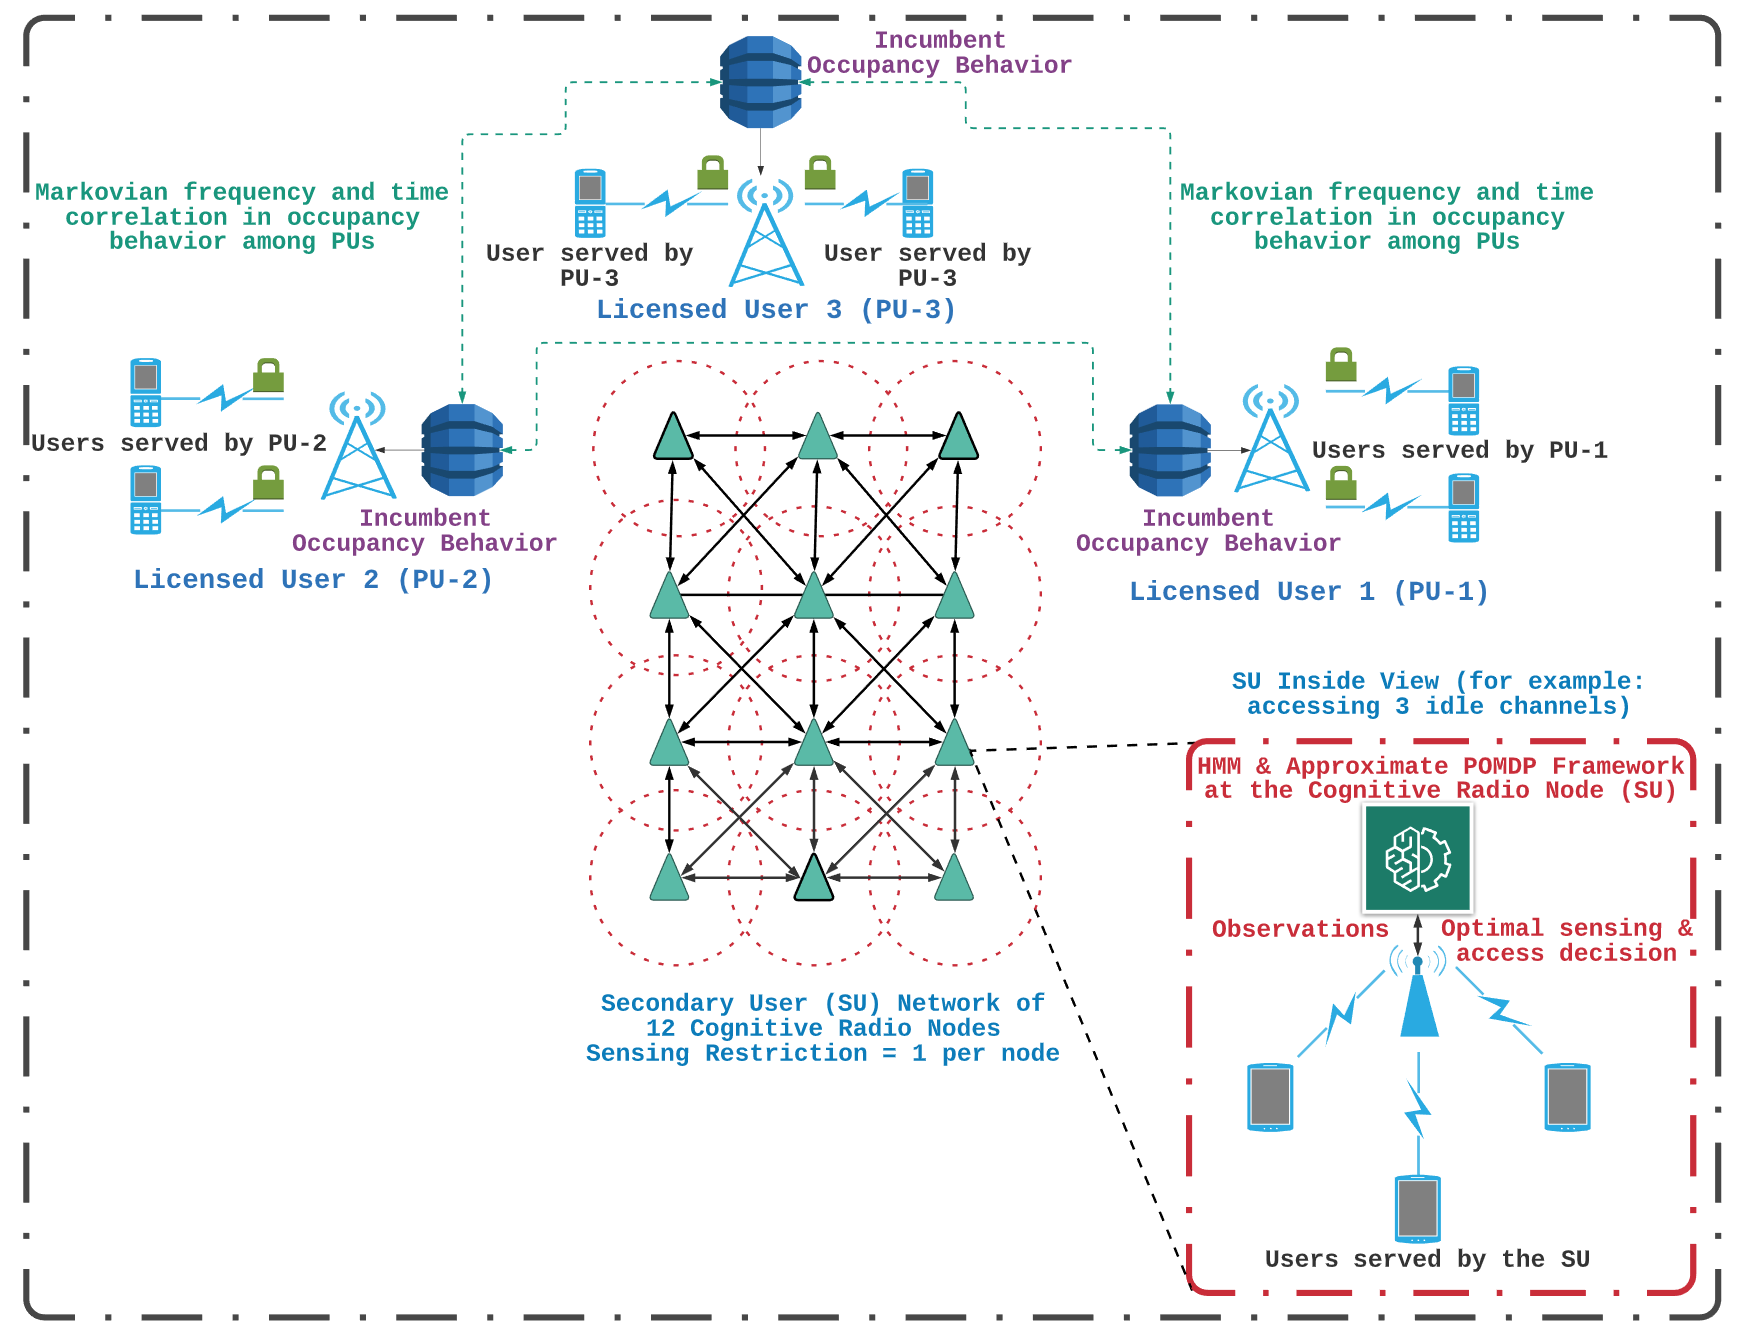
\includegraphics[width = 1.0\linewidth]{figures/Minerva_Multiagent_System_Model.png}}
    \vspace{-6mm}
    \caption{The radio ecosystem under analysis: An exemplification of the system model detailed in Sec. \ref{I.I} with $J{=}3$ and $\tilde{J}{=}12$: we first study deployment scenarios with $\tilde{J}{=}1$ before extending our analysis to multi-agent settings}
    \label{fig: A.0}
    \vspace{-7mm}
\end{figure}

\subsection{Occupancy Correlation Structure}\label{I.II}
The frequency domain signal of the PU occupying channel $k$ in time-slot $i$ is modeled as
\begin{equation}\label{3}
    X_{k}(i)=\sqrt{P_{T}}B_{k}(i)S_{k}(i),
\end{equation}
where $P_{T}$ denotes the transmission power of the occupant PU; $B_{k}(i)$ represents the binary channel occupancy variable, with $B_{k}(i){=}1$ if channel $k$ is occupied by a PU in time-slot $i$, and $B_{k}(i){=}0$ otherwise; $S_{k}(i)$ is the transmitted symbol, i.i.d across time and frequency, modeled from a certain constellation. Then, $H_{k}(i)X_{k}(i){=}\sqrt{P_{T}}B_{k}(i)H_{k}(i)S_{k}(i)$. Herein, we approximate $H_{k}(i)S_{k}(i)$ as a zero-mean complex Gaussian random variable with variance $\sigma_{H}^{2}\mathbb{E}[|S_{k}|^{2}]$. We denote the spectrum occupancy state in time-slot $i$ as
\begin{equation}\label{4}
    \vec{B}(i)=[B_{1}(i),B_{2}(i),B_{3}(i),\dots,B_{K}(i)]^{\intercal}{\in}\{0,1\}^{K}.
\end{equation}
We assume that spectrum occupancy is correlated in time and frequency because PUs typically occupy a set of adjacent channels (frequency correlation), repeating similar motifs in behavior over an extended period of time (temporal correlation) \cite{WCL:12, 4213046,McHenry:2006:CSO:1234388.1234389}. To capture temporal correlation, we model the evolution of $\vec{B}(i)$ over time as a Markov process
\begin{equation}\label{5}
    \mathbb{P}(\vec{B}(i+1)|\vec{B}(j),\forall j \leq i)=\mathbb{P}(\vec{B}(i+1)|\vec{B}(i)).
\end{equation}
In addition, to model frequency correlation, we further decompose $\mathbb{P}(\vec{B}(i+1)|\vec{B}(i))$ as
\begin{equation}\label{6}
    \mathbb{P}(\vec{B}(i+1)|\vec{B}(i))=\mathbb{P}(B_{1}(i+1)|B_{1}(i))\prod_{k=2}^{K}\mathbb{P}(B_{k}(i+1)|B_{k-1}(i+1),B_{k}(i)).
\end{equation}
In other words: the occupancy of frequency band $k$ in time-slot $i+1$ depends on the occupancy of the adjacent frequency band $k-1$ in the same time-slot $i+1$, and that of the same frequency band $k$ in the previous time-slot $i$,
as illustrated in Fig. \ref{fig:A.3}. If the frequency correlation direction is changed, i.e., the occupancy of channel $k+1$ influences the occupancy of channel $k$, $k{\in}\{1,2,...K{-}1\}$ (bottom-up correlation), our model and subsequent analyses still hold. We parameterize this two-chain Markovian correlation structure with the parameter vector $\vec{\theta}=[\vec{p}\ \vec{q}]^{\intercal}$, 
subsequently estimated with the Baum-Welch
in Sec. \ref{II.I},
where
\begin{equation}\label{7}
    \begin{aligned}
        \vec{p}&=[p_{uv}=\mathbb{P}(B_{k}(i+1)=1|B_{k-1}(i+1)=u,B_{k}(i)=v):u,v \in \{0,1\}]^{\intercal},\ \text{and}\\
        \vec{q}&=[q_{w}=\mathbb{P}(B_{1}(i+1)=1|B_{1}(i)=w):w \in \{0,1\}]^{\intercal}.
    \end{aligned}
\end{equation}
\begin{figure} [t]
    \centerline{
    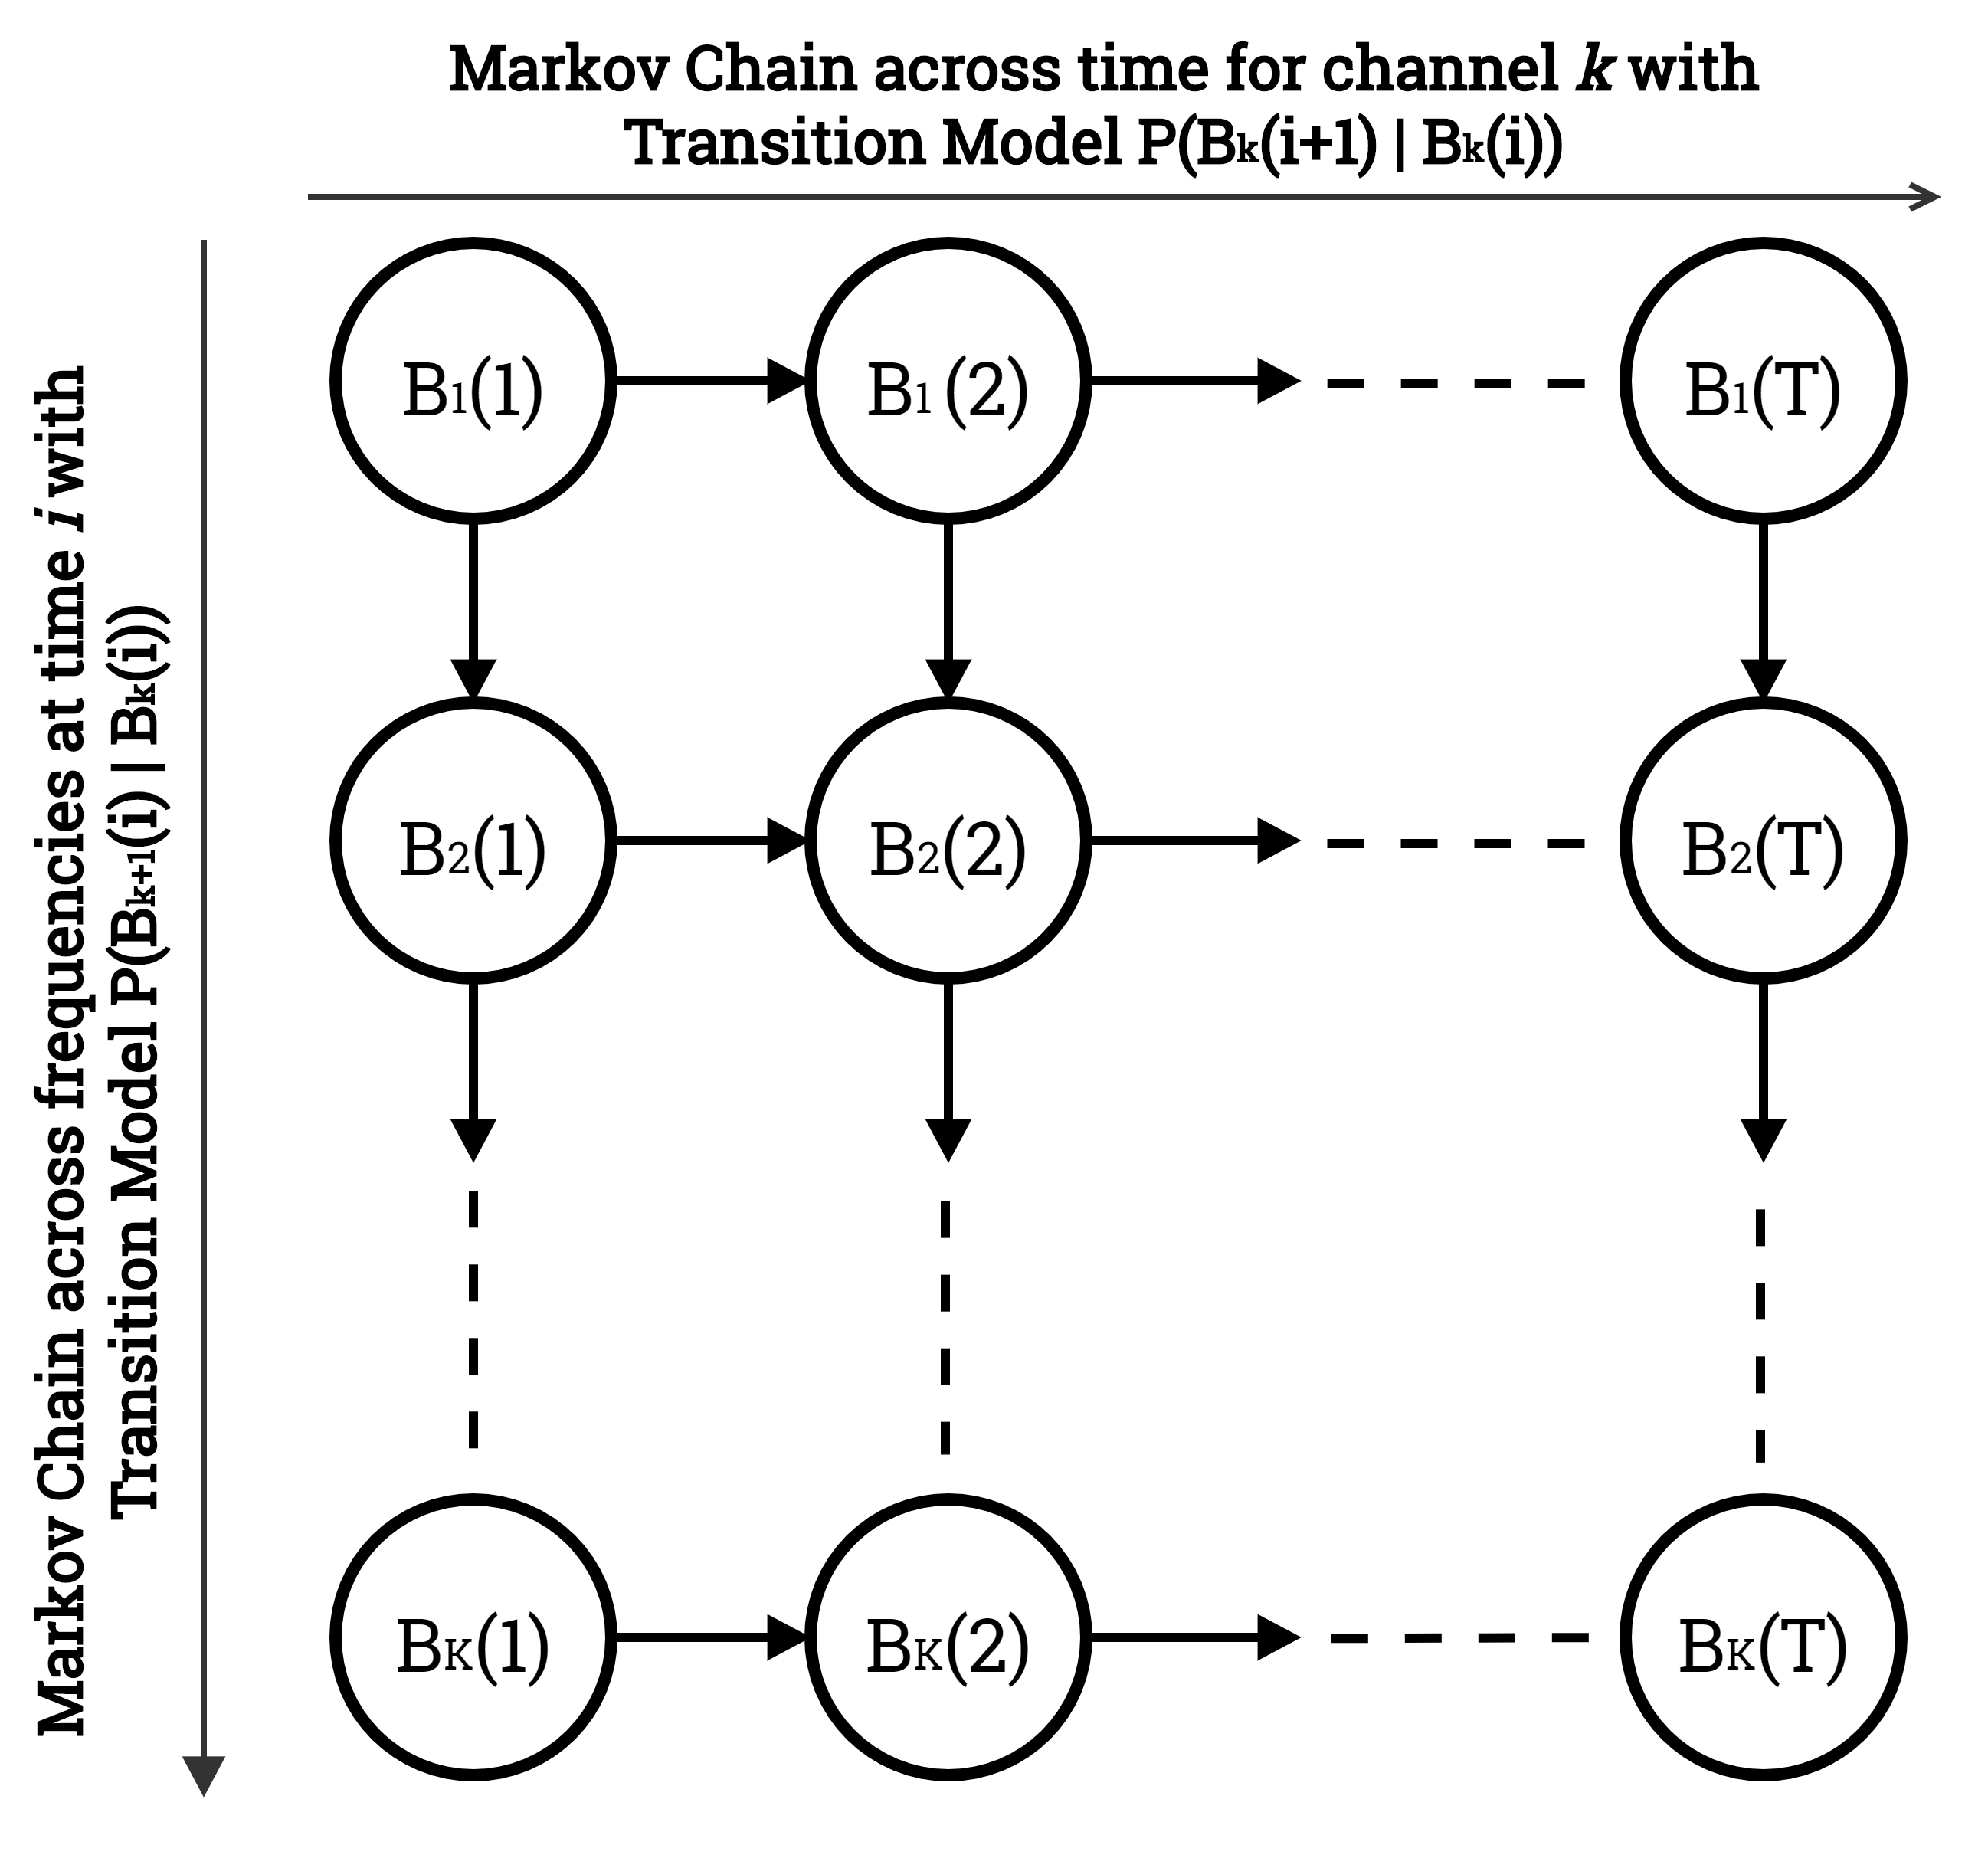
\includegraphics[width = 1.0\linewidth]{figures/Minerva_Occupancy_Markov_Chain_Flipped.png}}
    \vspace{-6mm}
    \caption{The visualization of the incumbent occupancy time-frequency correlation structure as two dependent Markov chains: one across time and the other across frequencies (L) | The combined PSD plot of the occupancy behavior of incumbents and competitors during the DARPA SC2 Active Incumbent scenario emulation (R)}
    \label{fig:A.3}
    \vspace{-7mm}
\end{figure}
To experimentally validate the proposed parameterized time-frequency correlated model, we  evaluated the Bayesian Information Criterion (BIC) metric,
defined as
\begin{equation}
\label{BIC}
   BIC = \gamma \ln{\nu} - 2\ln{\mathbb{P}(\mathbf{B}|\hat{\vec{\theta}}^*)},
\end{equation}
based on a dataset constituted of PSD measurements of the incumbent and the competitors in the DARPA SC2 Active Incumbent scenario emulated on the Colosseum \cite{DARPA:SC2, DARPA:SC2c2api, DARPA:ActiveIncumbent, DARPA:SC2scenarios}, depicted in Fig. \ref{fig:A.3} (R). In \eqref{BIC}, $\nu$ is the sample size, $\gamma$ is the number of model parameters, $\mathbf{B}$ is the time-frequency binary occupancy matrix from the dataset, and $\hat{\vec{\theta}}^*$ is the parameterized model fit to the dataset using the Baum-Welch algorithm detailed in Sec. \ref{II.I}. We used a 70-30 training-test split to evaluate the BIC metric, i.e., the occupancy data collected during the first $70$\% of the $330$ seconds of scenario emulation is used to estimate the model parameters, while the remaining $30$\% is employed to evaluate the BIC metric. We found that our proposed time-frequency correlation model yields a BIC of $72.061$, the best compared to other state-of-the-art models: time-frequency independence models ($98.868$) \cite{WCL:4, WCL:10, WCL:9, WCL:11, WCL:8}, only temporal correlation models ($95.257$) \cite{WCL:5}, and only frequency correlation models ($77.300$). This evaluation reveals that exploiting frequency correlation is more important than time correlation, but exploiting \emph{both} time and frequency correlation provides a better fit to the dataset.

\subsection{Channel Sensing Model}\label{I.III}
Equipped with a spectrum sensor, the SU detects white-spaces and accesses them to deliver its network flows. Due to concerns about energy-efficiency and sensing/data aggregation times \cite{WCL:3}, the SU can sense a maximum of $\kappa$ spectrum bands in a time-slot, with $1{\leq}\kappa{\leq}K$. Let $\mathcal{K}_{i}{\subseteq}\{1,2,\dots,K\}$ be the set of channels sensed by the SU at time $i$, with $|\mathcal{K}_{i}|{\leq}\kappa$. This selection is dictated by a sensing policy, as defined in Sec. \ref{II.II}. After sensing the channels listed in $\mathcal{K}_{i}$, the obtained observation vector is $\vec{Y}(i){=}[Y_{k}(i)]_{k{\in}\mathcal{K}_{i}}]$, with  $Y_{k}(i)$ given in \eqref{2}.

Owing to \eqref{2}, the  i.i.d. assumptions of the noise $V_{k}(i)$, the transmitted symbols $S_{k}(i)$, and the channels $H_{k}(i)$ across frequency, as discussed in Sec. \ref{I.I}, the probability density function (pdf) of $\vec{Y}(i)$ conditional on $\vec{B}(i)$ and the sensing set $\mathcal{K}_{i}$ is given by
\begin{equation}\label{8}
    f(\vec{Y}(i)|\vec{B}(i),\mathcal{K}_{i})=\prod_{k=1}^{K}f(Y_{k}(i)|B_{k}(i)),\text{ where }
        Y_{k}(i)|B_{k}(i)\sim\mathcal{CN}(0,\sigma_{H}^{2}P_{T}B_{k}(i)+\sigma_{V}^{2}).
\end{equation}

\subsection{POMDP Formulation}\label{II.0}
POMDPs model the repeated, sequential interactions of an agent tasked with maximizing its reward, with a stochastic environment, in which the agent has only access to noisy observations of the state. Our POMDP formulation, depicted in Fig. \ref{fig: A.add-1} and
represented by the 5-tuple $(\mathcal{B},\mathcal{A},\mathcal{Y},\mathbf{A},\mathbf{M})$, features the state space of the underlying MDP, denoted by $\mathcal{B}{\equiv}\{0,1\}^{K}$, which is given by all possible realizations of the occupancy vector $\vec{B}$; the action space of the SU, denoted by $\mathcal{A}$, which is described by all possible combinations in which $1{\leq}\kappa{\leq}K$ channels are chosen to be sensed in a time-slot (discussed in Sec. \ref{I.III}); the observation space, denoted by $\mathcal{Y}$, which is discussed in Sec. \ref{I.I}; the transition model of the underlying MDP, denoted by $\mathbf{A}$, which is discussed in Sec. \ref{I.II}; and the observation model (also known as the emission model), denoted by $\mathbf{Y}$, and described by \eqref{8}. The POMDP process flow, relevant to our discussions in this section, is illustrated in Fig. \ref{fig: A.add-1}.
\begin{figure} [t]
    \centerline{
    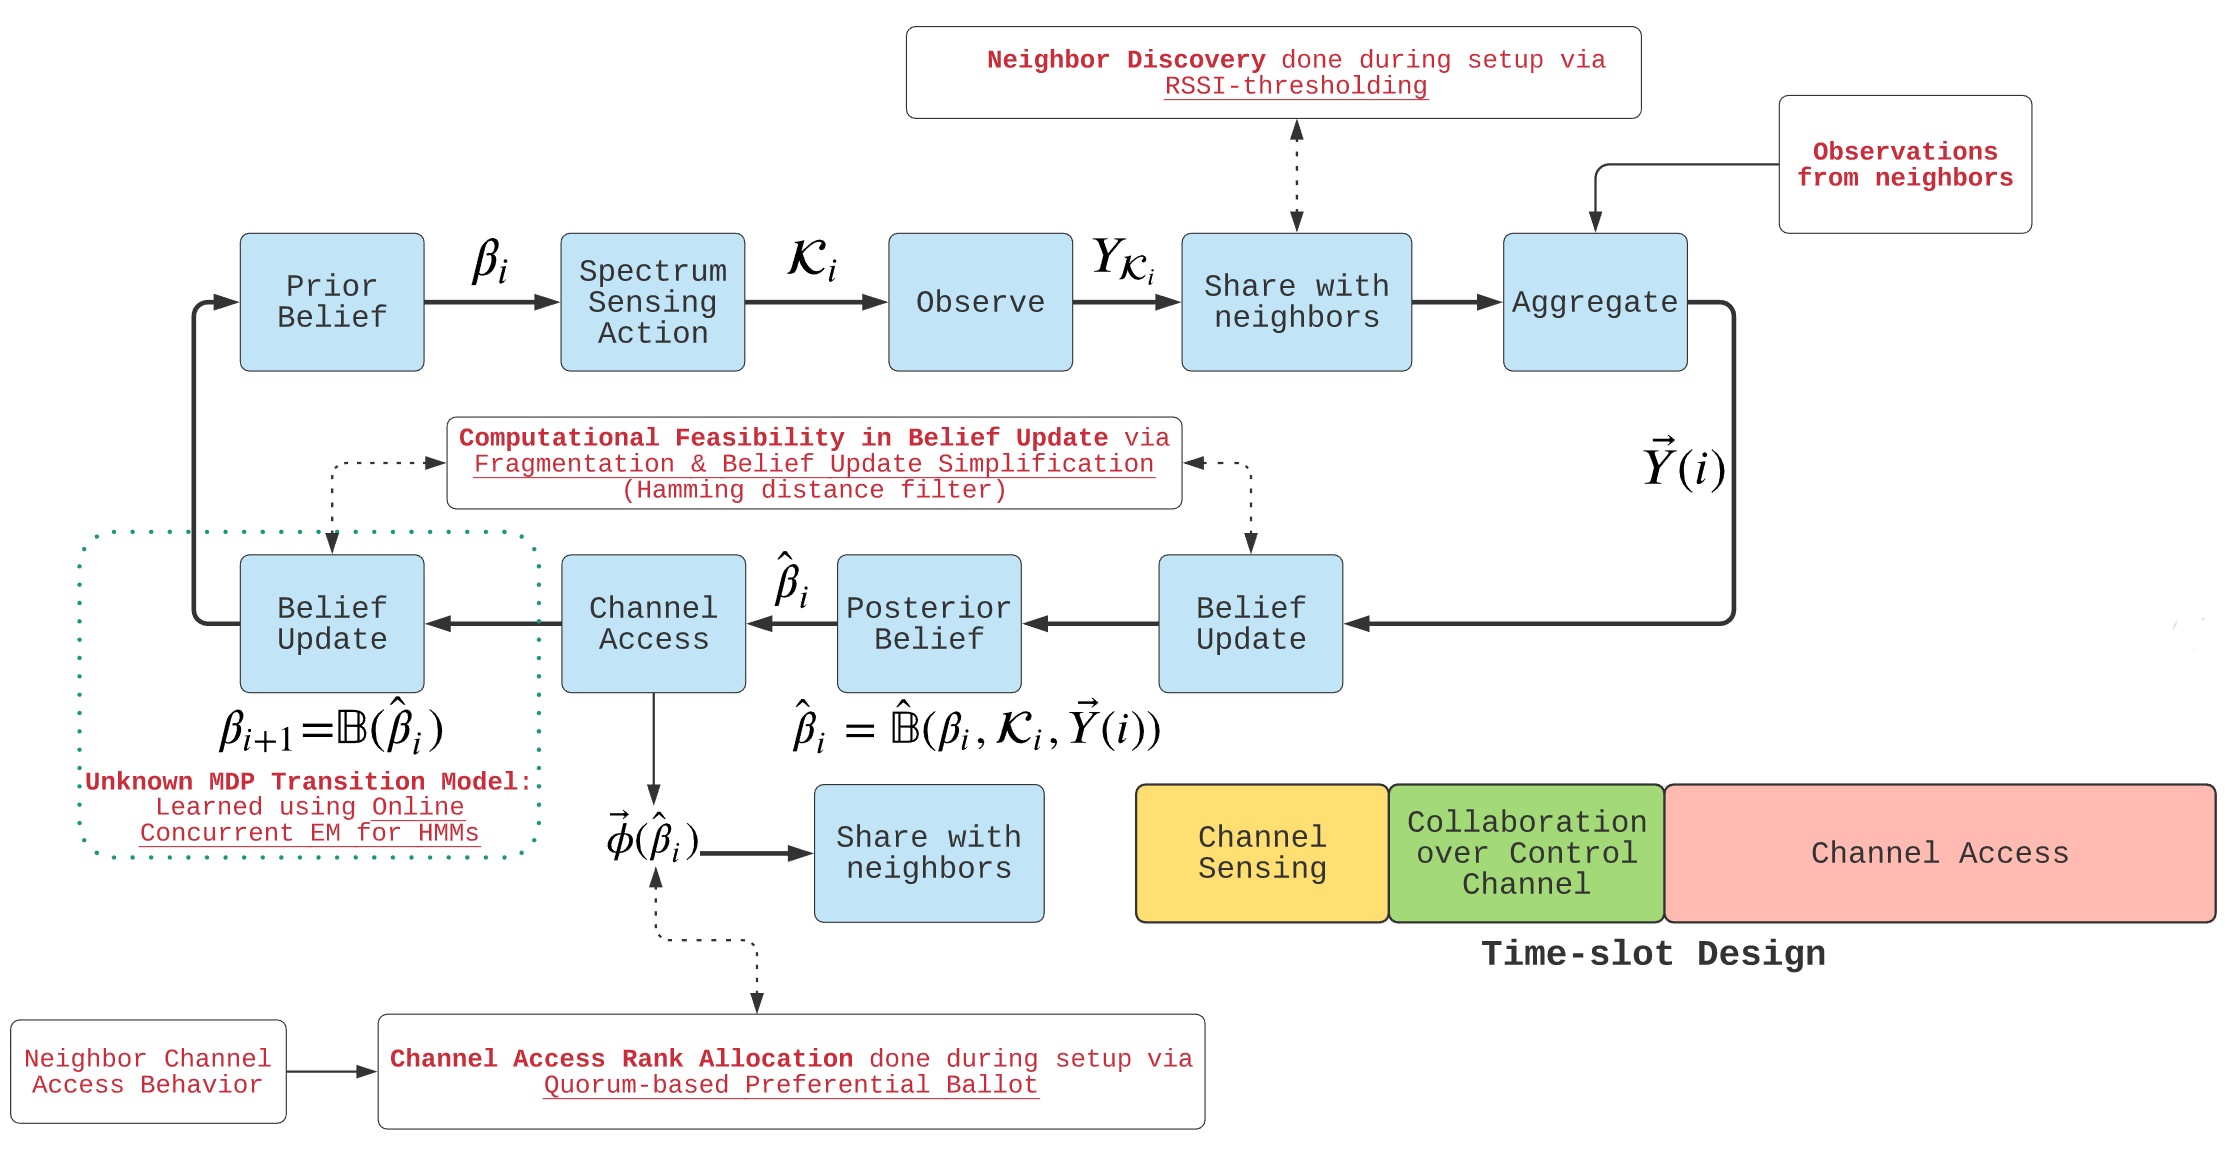
\includegraphics[width = 1.0\linewidth]{figures/POMDP_MultiAgent_Model.PNG}}
    \vspace{-6mm}
    \caption{The POMDP process flow as discussed in Sec. \ref{II.0}, with neighbor discovery, channel access rank allocation, and time-slot design being relevant design points discussed in our multi-agent deployment analysis (Sec. \ref{Z})}
    \vspace{-7mm}
    \label{fig: A.add-1}
\end{figure}

Prior to gathering the occupancy information in time-slot $i$, based on the measurements obtained by the SU's spectrum sensor up to, but not including, time-slot $i$, the POMDP state is described by the prior belief, denoted by $\beta_{i}$, representing the probability distribution of the underlying MDP state $\vec{B}(i)$ given the history. Given $\beta_{i}$, the SU chooses a sensing action according to a sensing policy $\mathcal{K}_{i}=\pi(\beta_{i}){\in}\mathcal{A}$, 
senses the frequency bands corresponding to the channel indices in the set $\mathcal{K}_{i}$ (Sec. \ref{I.III}), observes $[Y_{k}(i)]_{k{\in}\mathcal{K}_{i}}{\in}\mathcal{Y}$, and updates its belief of the underlying MDP state $\vec{B}(i)$ to obtain the posterior belief
\begin{equation}\label{10}
    \begin{aligned}
        \hat{\beta}_{i}(\vec{B}')&=\mathbb{P}(\vec{B}(i)=\vec{B}'|\beta_{i},\mathcal{K}_{i},[Y_{k}(i)]_{k{\in}\mathcal{K}_{i}})\\
        &=\frac{\mathbb{P}([Y_{k}(i)]_{k{\in}\mathcal{K}_{i}}|\vec{B}',\mathcal{K}_{i})\beta(\vec{B}')}{\sum_{\vec{B}'' \in \{0,1\}^{K}}\mathbb{P}([Y_{k}(i)]_{k{\in}\mathcal{K}_{i}}|\vec{B}'',\mathcal{K}_{i})\beta_{i}(\vec{B}'')}.
    \end{aligned}
\end{equation}
Given  $ \hat{\beta}_{i}$ the SU then performs channel access decisions
$\vec{\phi}(i)\in\{0,1\}^K$, where
$\vec{\phi}_k(i)=1$ if the SU accesses the $k$th spectrum band, and $\vec{\phi}_k(i)=0$ otherwise. To determine $\vec{\phi}(i)$, we define the expected reward metric
\begin{equation}\label{12}
    R(\vec{\phi}(i),\hat{\beta}_{i})=\sum_{k=1}^{K}(1-\hat{\beta}_{i,k})\phi_{k}(i)-\lambda \hat{\beta}_{i,k}\phi_k(i).
\end{equation}
Note that, if the SU uses the $k$th spectrum band ($\phi_{k}(i)=1$), it accrues a reward if the
spectrum band is truly idle (with posterior probability $1-\hat{\beta}_{i,k}$), and a penalty $\lambda$ if it is occupied (with posterior probability $\hat{\beta}_{i,k}$); it accrues no reward for not using a channel. Hence, this reward metric captures both the number of truly idle channels (correctly estimated idle) accessed by the cognitive radio, accounting for the throughput maximization aspect of our objective, as well as the number of truly occupied channels (incorrectly estimated idle) accessed by it, accounting for the incumbent interference minimization aspect of our objective, where $\lambda$ regulates such trade-off. The optimal access decision is $\vec{\phi}^{*}(i){=}\arg\max R(\vec{\phi}(i),\hat{\beta}_{i})$, which can be solved in closed form as
\begin{equation}
    \phi_{k}^{*}(i) = \left\{
        \begin{array}{cc}
             1, &  \hat{\beta}_{i}{<}\frac{1}{1{+}\lambda}\\
             0, &  \text{otherwise}
        \end{array}\right.
\end{equation}
yielding the optimal reward
$$
R^*(\hat{\beta}_{i})=\max_{\vec{\phi}\in\{0,1\}^K} R(\vec{\phi}(i),\hat{\beta}_{i})
=
\sum_{k=1}^{K}\max\{1-(1+\lambda)\hat{\beta}_{i,k},0\}.
$$
In other words, if the agent is confident that the channel is idle ($\hat{\beta}_{i}{<}\frac{1}{1{+}\lambda}$), then the SU accesses it; otherwise, it remains idle.

Ensuing the determination of the reward for its access decision from the radio environment, the SU computes the prior belief for the next time-slot $i+1$ as
\begin{equation}\label{13}
    \beta_{i+1}(\vec{B}'')=\sum_{\vec{B}'}\mathbb{P}(\vec{B}(i+1)=\vec{B}''|\vec{B}(i)=\vec{B}')\hat{\beta}(\vec{B}').
\end{equation}
Let
\begin{equation}\label{14}
    \hat{\beta}_{i}=\hat{\mathbb{B}}(\beta_{i},\mathcal{K}_{i},\vec{Y}(i)),\ \ \ \beta_{i+1}=\mathbb{B}(\hat{\beta}_{i})
\end{equation}
denote the functions that map the prior belief $\beta_{i}$ to the posterior belief $\hat{\beta}_{i}$ in time-slot $i$, and the posterior belief $\hat{\beta}_{i}$ to the next prior belief $\beta_{i+1}$ in time-slot $i+1$ . The objective of the SU is to determine the optimal spectrum sensing policy (based on which the access decisions are made in the corresponding time-slots) to maximize its infinite-horizon discounted reward, i.e.,
\begin{equation}\label{16}
    \pi^{*}=\argmax_{\pi}V^{\pi}(\beta),
\end{equation}
where
\begin{equation}\label{17}
    V^{\pi}(\beta)=\mathbb{E}_{\pi}\left[\sum_{i=1}^{\infty}\gamma^{i}
    R^*(\hat{\beta}_{i})\Big{|}\beta_{0}=\beta\right],
\end{equation}
where $0{<}\gamma{<}1$ is the discount factor, $\beta_{0}{=}\beta$ is the initial belief, and $\hat{\beta}_{i}$ is the posterior belief induced by the policy $\mathcal{K}_{i}{=}\pi(\beta_{i})$ and the observation vector $[Y_{k}(i)]_{k{\in}\mathcal{K}_{i}}$ via $\hat{\beta}_{i} = \hat{\mathbb{B}}(\beta_{i}, \mathcal{K}_{i} = \pi(\beta_{i}), [Y_{k}(i)]_{k \in \mathcal{K}_{i}})$. The optimal value function $V^*(\beta)$ can be shown to be solution of the Bellman's optimality equation $V^{*}{=}\mathcal{H}(V^{*})$ \cite{PUOccupancy:18}, where $\mathcal H$ is the Bellman's operator, defined as $V_{t+1}{=}\mathcal{H}(V_t)$ with
\begin{equation}\label{18}
    \begin{aligned}
        V_{t+1}(\beta)
        =\max_{\mathcal{K} \in \mathcal{A}}\sum_{\vec{B} \in \mathcal{B}}\beta(\vec{B})\mathbb{E}_{[Y_{k}]_{k \in \mathcal{K}}|\vec{B},\mathcal{K}}\left[R^*(\hat{\mathbb{B}}(\beta,\mathcal{K},[Y_{k}]_{k \in \mathcal{K}}))+\gamma V_{t}(\mathbb{B}(\hat{\mathbb{B}}(\beta,\mathcal{K},[Y_{k}]_{k \in \mathcal{K}}))\right],\ \forall \beta.
    \end{aligned}
\end{equation}
The optimal value function $V^*$ can be determined via the value iteration algorithm
$V_{t+1}=\mathcal H(V_t)$, which converges to  $V^*$ as $t\to\infty$ \cite{PUOccupancy:18}. However, this direct approach results in complications associated with the lack of prior knowledge about the incumbent occupancy time-frequency correlation structure that defines the transition model of the underlying MDP, and the computational infeasibility of the approach: as the number of channels in the discretized spectrum of interest increases, the number of states of the underlying MDP scales exponentially, resulting in a high-dimensional belief space, which makes the approach intractable. To address these two challenges, we propose the following solutions:
\begin{itemize}
    \item We incorporate an HMM EM estimator, i.e., the Baum-Welch algorithm, to learn the time-frequency occupancy correlation structure while concurrently solving for the optimal sensing and access policy. This is developed in Sec. \ref{II.I}.
    \item We incorporate a low-complexity approximate value iteration algorithm known as PERSEUS \cite{WCL:13}, with fragmentation (into independent subsets of highly-correlated channels) and belief update simplification heuristics (Hamming distance state filters). This is developed in Sec. \ref{II.II}.
\end{itemize}

\section{Proposed Solution: The Algorithms}\label{II}
Practical MAC layer implementations of cognitive radios involve solving for the optimal sensing and access policy, without having any prior information about the time-frequency correlation structure underlying the occupancy behavior of the incumbents in the network. \cite{8935729, 8935774}. As discussed earlier, this correlation structure may be leveraged to improve  white-space detection, hence utilization. In this section, we propose a parameter estimator algorithm that learns this correlation structure over time. In Sec. \ref{II.II}, we then use this knowledge in an approximate
point-based value iteration framework based on PERSEUS \cite{WCL:13} to determine the optimal sensing and access policy. Crucially, the parameter estimation and PERSEUS algorithms are executed concurrently, which is especially vital in non-stationary settings.

\subsection{Occupancy Correlation Structure Estimation}\label{II.I}
Let $\tau$ refer to the learning period of the parameter estimation algorithm: this can be equal to the entire duration of the SU's interaction with the radio environment while solving for the optimal policy, implying concurrent model learning, or it can  be equal to an initial learning period that has been set aside exclusively for the SU to estimate the underlying MDP's transition model, after which the PERSEUS algorithm is initiated, employing these final estimated (converged) transition probabilities. Defining $\mathbf{B}{=}[\vec{B}(i)]_{i{=}1}^{\tau}$ as the unknown sequence of states and $\mathbf{Y}{=}[\vec{Y}(i)]_{i{=}1}^{\tau}$ as the sequence of observations made at the SU's spectrum sensor from $i{=}1$ to $i{=}\tau$, we formulate the Maximum Likelihood Estimation (MLE) problem to estimate the vector $\vec{\theta}$ that parameterizes the PU occupancy time-frequency correlation structure (detailed in Sec. \ref{I.II}) as
\begin{equation}\label{19}
    \vec{\theta}^{*}=\argmax_{\vec{\theta}}\log{\left(\sum_{\mathbf{B}}\mathbb{P}(\mathbf{B},\mathbf{Y}|\vec{\theta})\right)}.
\end{equation}
Solving this MLE formulation using the Baum-Welch algorithm, an Expectation-Maximization algorithm for HMMs \cite{WCL:14}, the E-step constitutes
\begin{equation}\label{20}
    Q(\vec{\theta}|\vec{\theta}^{(t)})=\mathbb{E}_{\mathbf{B}|\mathbf{Y},\vec{\theta}^{(t)}}\left[\log{(\mathbb{P}(\mathbf{B},\mathbf{Y}|\vec{\theta}^{(t)})}\right],
\end{equation}
which can be computed using the Forward-Backward algorithm \cite{WCL:14}; and the M-step constitutes
\begin{equation}\label{21}
    \vec{\theta}^{(t+1)}=\argmax_{\vec{\theta}}Q(\vec{\theta}|\vec{\theta}^{(t)}),
\end{equation}
which involves the re-estimation of $\vec{\theta}$ by employing the statistics $Q(\vec{\theta}|\vec{\theta}^{(t)})$ obtained from the Forward-Backward algorithm \bk{Equations?}.

\subsection{The PERSEUS Algorithm}\label{II.II}
In our proposed solution, we solve for the optimal spectrum sensing (and access, based on reward maximization detailed in Sec. \ref{II.0}) policy, in parallel with the parameter estimation algorithm, employing its published iterative transition model estimates, until both the EM algorithm and the POMDP policy solver algorithms converge.

As alluded to in Sec. \ref{II.0}, in order to solve the computational infeasibility precipitated by the exponential increase in the number of states of the underlying MDP, induced by an increase in the number of frequency bands in the discretized spectrum of interest, we employ approximate POMDP value iteration methods to ensure that the formulations and the algorithms scale well to a large number of relevant channels in the radio environment in which the SU operates. We choose the PERSEUS algorithm \cite{WCL:13} to solve for the optimal policy, primarily motivated by the following: the exact value iteration strategies proposed in \cite{PUOccupancy:18}, namely the Exhaustive Enumeration algorithm and the Witness algorithm are untenable for large belief spaces, because these techniques involve performing the backup procedure, i.e., determining the optimal action (or hyperplane in a Piece-Wise Linear Convex (PWLC) context) for every belief point in the belief space; and a fellow contemporary approximate value iteration algorithm known as the Point-Based Value Iteration (PBVI) algorithm proposed in \cite{PUOccupancy:17}, although involves performing the backup operation over a reduced set of beliefs known as the "reachable beliefs," unlike the strategies in \cite{PUOccupancy:17}, is computationally expensive due to the task of computing the distances between all the belief points in the set of reachable beliefs in addition to the subsequent backup operation on all these belief points. The PERSEUS algorithm, on the other hand, does not involve performing the backup operation for every point in the belief space, unlike the Exhaustive Enumeration and Witness algorithms detailed in \cite{PUOccupancy:18}; and unlike the PBVI algorithm \cite{PUOccupancy:17} does not involve computing the distances between all the belief points in the set of reachable beliefs, and furthermore, does not involve performing backups on all the reachable belief points, instead, PERSEUS involves "backing-up" only on a subset of this set of reachable beliefs, while ensuring that the computed solution is effective for all the points in the reachable belief set.

PERSEUS, a randomized, point-based, approximate POMDP value iteration algorithm, involves an initial phase of exploration, wherein the set of "reachable-beliefs," denoted by $\tilde{\mathcal{B}}$, is determined by allowing the SU to randomly interact with the radio environment. As referenced earlier, one simplifying (or approximating) feature of PERSEUS is to improve the value of all the belief points in the set $\tilde{\mathcal{B}}$, by computing the value of only a subset of these belief points, which are chosen iteratively at random. For finite-horizon POMDP formulations, the optimal value function $V^{*}$ described by \eqref{18}, can be approximated by a Piece-Wise Linear Convex (PWLC) function \cite{WCL:13}, in other words, the value function at iteration $t$ is parameterized by a set of hyperplanes, denoted by $\{\vec{\alpha}_{t}^{u}\},u{\in}\{1,2,\dots,|\tilde{\mathcal{B}}|\}$, wherein each hyperplane represents a region of the belief space for which the action corresponding to this hyperplane, denoted by $\mathcal{K}_{t}^{u}$, is the maximizer. Ergo, the value function of belief $\beta$ in a given iteration $t$ is approximated as
\begin{equation}\label{22}
    V_{t}(\beta) \approx \beta \max_{u \in \{1,2,\dots,|\tilde{\mathcal{B}}|\}} \cdot \vec{\alpha}_{t}^{u},
\end{equation}
where
\begin{equation}\label{24}
    \beta \cdot \vec{\alpha}=\sum_{\vec{B}}\beta(\vec{B})\vec{\alpha}(\vec{B})
\end{equation}
denotes inner product.
The approximately optimal spectrum sensing action
is the one associated with the minimizing hyperplane $\alpha^*$,
and denoted as $\mathcal{K}_{t}^{u^{*}}$.

We define a set of unimproved belief points, denoted as $\tilde{\mathcal{U}}$, which initially corresponds to the set of reachable beliefs $\tilde{\mathcal{B}}$ obtained by the random exploration procedure detailed earlier. Pick a belief $\beta_{u}$ from this set $\tilde{\mathcal{U}}$, and perform the backup operation on this chosen belief point, which as discussed earlier, involves associating a new hyperplane and its corresponding spectrum sensing action with this belief $\beta_{u}$. In iteration $t+1$, defining $\mathcal{K}_{t+1}^{u}$ as the action associated with hyperplane $\vec{\alpha_{t+1}}$, corresponding to belief $\beta_{u}{\in}\tilde{\mathcal{U}}$, we can describe the backup procedure mathematically as
\begin{equation}\label{25}
    \begin{aligned}
        \vec{\alpha}_{t+1}&=\xi_{\mathcal{K}_{t+1}^{u}}^{u},\\
        \mathcal{K}_{t+1}^{u}&=\argmax_{\mathcal{K} \in \mathcal{A}}\beta_{u} \cdot \xi_{\mathcal{K}}^{u},
    \end{aligned}
\end{equation}
where $\xi_{\mathcal{K}}^{u}$ is the hyperplane corresponding to the one-step look-ahead under action $\mathcal{K}{\in}\mathcal{A}$ and belief $\beta_{u}$, i.e.,
\begin{equation}\label{26}
    \xi_{\mathcal{K}}^{u}(\vec{B})=\mathbb{E}_{\vec{Y}|\vec{B},\mathcal{K}}\left[R(\vec{B},\hat{\mathbb{B}}(\beta_{u},\mathcal{K},\vec{Y}))+\gamma \sum_{\vec{B}'}\mathbb{P}(\vec{B}(i+1)=\vec{B}'|\vec{B}(i)=\vec{B})\xi_{\mathcal{K},\vec{Y}}^{u}(\vec{B}')\right],
\end{equation}
where $\xi_{\mathcal{K},\vec{Y}}^{u}$ refers to the hyperplane corresponding to the future value function computed from the previous set of hyperplanes from the new belief $\mathbb{B}(\hat{\mathbb{B}}(\beta_{u},\mathcal{K},\vec{Y}))$ obtained from $\beta_{u}$ by executing action $\mathcal{K}$ and observing $\vec{Y}$, as
\begin{equation}\label{27}
    \xi_{\mathcal{K},\vec{Y}}^{u}=\argmax_{\vec{\alpha}_{t}^{u'},u' \in \{1,2,\dots,|\tilde{\mathcal{B}}\}}\mathbb{B}(\hat{\mathbb{B}}(\beta_{u},\mathcal{K},\vec{Y})) \cdot \vec{\alpha}_{t}^{u'}.
\end{equation}

After determining the hyperplane $\alpha_{t+1}^{u}$ associated with this chosen belief point $\beta_{u}$ using the backup procedure detailed above, we now know that $V_{t+1}(\beta_{u}){=}\beta_{u}{\cdot}\vec{\alpha}_{t+1}^{u}$ is its approximate value function. The most crucial aspect of PERSEUS that approximates the optimization of a randomly chosen belief point to the entire set $\tilde{\mathcal{U}}$ is as follows: if the approximate value function for belief point $\beta_{u}{\in}\tilde{\mathcal{U}}$ is improved by the aforementioned backup iteration, i.e., $V_{t+1}(\beta_{u}){\geq}V_{t}(\beta_{u})$, the belief point $\beta_{u}$ is removed from the set $\tilde{\mathcal{U}}$, and now, we check if this hyperplane $\vec{\alpha}_{t+1}^{u}$ improves the approximate value functions of the other beliefs in $\tilde{\mathcal{U}}$, i.e., ${\forall}\beta'{\in}\tilde{\mathcal{U}}{-}\{\beta_{u}\}$, if $\beta'{\cdot}\vec{\alpha}_{t+1}^{u}{\geq}V_{t}(\beta')$, this new hyperplane generates an improved approximate value function, and these respective belief points for which this hyperplane improves their approximate value functions, are removed from the set $\tilde{\mathcal{U}}$. In other words,
\begin{equation}\label{28}
    \begin{aligned}
        \tilde{\mathcal{U}} &\longleftarrow \tilde{\mathcal{U}}-\{\beta_{u}\},\text{ if }\beta_{u}{\cdot}\vec{\alpha}_{t+1}^{u} \geq V_{t}(\beta_{u}),\text{ and subsequently}\\
        \tilde{\mathcal{U}} &\longleftarrow \tilde{\mathcal{U}}-\{\beta' \in \tilde{\mathcal{U}}:\beta' \cdot \vec{\alpha}_{t+1}^{u} \geq V_{t}(\beta')\}.
    \end{aligned}
\end{equation}

On the other hand, if this hyperplane $\vec{\alpha}_{t+1}^{u}$ worsens the approximate value function of $\beta_{u}$, i.e., $\beta_{u}{\cdot}\vec{\alpha}_{t+1}^{u}{<}V_{t}(\beta_{u})$, the old hyperplane and its associated sensing action persist for $\beta_{u}$, mathematically, $\vec{\alpha}_{t+1}^{u}{:=}\vec{\alpha}_{t}^{u}$ and $\mathcal{K}_{t+1}^{u}{:=}\mathcal{K}_{t}^{u}$; but we still check for improvements with respect to the other belief points in $\tilde{\mathcal{U}}$, and remove all those belief points $\beta'{\in}\tilde{\mathcal{U}}$ for which $\beta'{\cdot}\vec{\alpha}_{t+1}^{u}{\geq}V_{t}(\beta')$. 

In general, if a hyperplane determined from the backup procedure improves a belief point in the set of unimproved belief points $\tilde{\mathcal{U}}$, this news hyperplane (and its associated sensing action) becomes the relevant hyperplane (and the relevant sensing action) for this belief point, and the belief point will be removed from the set of unimproved belief points $\tilde{\mathcal{U}}$. These sequence of operations (random choice from $\tilde{\mathcal{U}}$ ${\longrightarrow}$ backup ${\longrightarrow}$ check for improvement and removal) are performed iteratively until the set $\tilde{\mathcal{U}}$ is empty: this constitutes a single PERSEUS iteration. These PERSEUS iterations are executed until the specified value iteration termination condition is satisfied, i.e.,
\begin{equation}\label{29}
    |V_{t+1}(\beta)-V_{t}(\beta)|<\epsilon,\ \forall \beta \in \tilde{\mathcal{B}},
\end{equation}
where $\epsilon{>}0$ (a very small value), is the value iteration difference threshold.

The PERSEUS algorithm, although is an approximate POMDP method which eliminates the computational overhead associated with the exhaustive belief space and reachable space optimization techniques \cite{PUOccupancy:18,PUOccupancy:17} by approximating the optimization of a randomly chosen belief point to the entire set of unimproved, reachable belief points, still possesses computational intractability challenges because it involves iterations over all possible combinations of the occupancy state vector, i.e., $\vec{B}{\in}\{0,1\}^{K}$, the computational cost scales exponentially with the number of states in the underlying MDP, which is induced by the number of channels $K$ in the discretized spectrum of interest. In order to solve this computational tractability problem, we introduce two simplifying heuristics into the PERSEUS algorithm. Firstly, we avoid iterating over all possible occupancy states by considering only those state transitions that involve a Hamming distance of $d{\in}\{1,2,\dots,K\}$ between two consecutive state vectors, $\vec{B}(i)$ and $\vec{B}(i+1)$,this is practical because the temporal dynamics of the occupancy of the radio environment, dictated by the behavior of the PUs in the network, are typically slower than the processing dynamics of the POMDP agent, i.e., the SU. Secondly, we fragment the discretized spectrum into smaller, independent sets of correlated channels (for example, an $18$ channel radio environment with $3$ PUs is fragmented into $3$ independent fragments, each comprising $6$ channels correlated by the occupancy behavior of the corresponding PU); run PERSEUS on these fragments concurrently by employing multi-threading capabilities in software frameworks; and finally, combine the results from each of these fragmented, parallel runs to get a full picture about the performance of our POMDP agent: this is practical because in a radio environment with multiple PUs, each PU is typically restricted to a portion (a set of adjacent frequency bands) of the spectrum, either by design or by bureaucracy.

\section{Numerical Evaluations}\label{III}
Sticking with the single-agent deployment setting, our simulations evaluate the operational capabilities of the proposed POMDP framework and compare it against the state-of-the-art. The simulated radio environment constitutes $J{=}3$ incumbents, i.e., PUs, accessing a $2.88$ MHz spectrum, discretized into $K{=}18$ channels, each having a bandwidth of $W{=}160$ kHz, and a cognitive radio node ($\tilde{J}{=}1$ SU) trying to intelligently access spectrum holes to deliver its network flows while limiting incumbent interference, as illustrated in Fig. \ref{fig: A.0}. The $3$ PUs access these $18$ channels according to a time-frequency Markovian correlation structure parameterized by
\[\vec{\theta}=\begin{bmatrix}
                    \vec{p} & \vec{q}
               \end{bmatrix}\]
as described in Sec. \ref{I.II}, where
\[\vec{p}=\begin{bmatrix}
            p_{00}=0.1 & p_{01}=0.3 & p_{10}=0.3 & p_{11}=0.7
          \end{bmatrix},\]
and
\[\vec{q}=\begin{bmatrix}
            q_{0}=0.3 & q_{1}=0.8
          \end{bmatrix}.\]

Regarding the channel sensing limitations induced by a need to minimize the amount of time and energy spent sensing the spectrum \cite{WCL:3}, we model our simulation framework on $\kappa{=}6$, i.e., in any given time-slot $i$, the SU can sense a maximum of $6$ channels out of the $18$ in the discretized spectrum of interest. Regarding the expected Signal to Interference Noise Ratios (SINR) at the PUs and the SU, subject to fading, and conditioned on the PU and SU access decisions, we model our simulation framework based off the following numbers:
\begin{align*}
    &\text{SINR}_{\text{SU}}(k,i){=}0,\text{if the SU does not access channel $k$ in time-slot $i$,}\\
    &\text{SINR}_{\text{SU}}(k,i){=}11\ \text{dB},\text{if the SU accesses a truly idle channel $k$ in time-slot $i$,}\\
    &\text{SINR}_{\text{SU}}(k,i){=}{-}6\ \text{dB},\text{if SU accesses an incumbent-occupied channel $k$ in slot $i$,}\\
    &\text{SINR}_{\text{PU}_{j}}(k,i){=}0,\text{if the PU $j$ does not access channel $k$ in time-slot $i$,}\\
    &\text{SINR}_{\text{PU}_{j}}(k,i){=}17\ \text{dB},\text{if PU $j$ occupies channel $k$ in slot $i$ without SU interference,}\\
    &\text{SINR}_{\text{PU}_{j}}(k,i){=}6\ \text{dB},\text{if PU $j$ occupies channel $k$ in slot $i$ with SU interference.}
\end{align*}

As described in Sec. \ref{I}, the only objective of the SU is to maximize its throughput subject to a constraint on the amount of interference its transmissions can cause to incumbents in the network. To this end, assuming an always back-logged SU, i.e., the SU always has network flows to deliver, the optimal POMDP sensing policy dictates which channels should be sensed by the SU's spectrum sensor in a given time-slot, based off the learned correlated occupancy dynamics of the PUs, in order to obtain an optimal picture about the occupancy of the channels in this time-slot, and then access all the channels deemed to be idle by the reward maximization procedure detailed in Sec. \ref{II.0}. The average throughput attained by the SU over $T$ time-slots is given by
\begin{equation}\label{30}
    C^{\text{SU}}=\frac{1}{T}\sum_{i=1}^{T}\sum_{k=1}^{K}R_{\text{SU}}\mathcal{I}\left\{\text{SINR}_{\text{SU}}(k,i) \geq 2^{\frac{R_{\text{SU}}}{W}}-1\right\},
\end{equation}
where $R_{\text{SU}}{=}0.6$ Mbps is the transmission rate of the SU on each channel, and $\mathcal{I}$ is an indicator variable; and the throughput attained by the PUs in the network over the same $T$ time-slots, normalized over time and the number of transmissions (normalization is necessary here because of the temporally intermittent transmissions of the PUs, the PUs are not always back-logged, unlike the SU) is given by
\begin{equation}\label{31}
    C^{\text{PUs}}=\frac{\sum_{i=1}^{T}\sum_{k=1}^{K}R_{\text{PU}}B_{k}(i)\mathcal{J}\left\{\text{SINR}_{\text{PU}}(k,i) \geq 2^{\frac{R_{\text{PU}}}{W}}-1\right\}}{\sum_{i=1}^{T}\sum_{k=1}^{K}B_{k}(i)},
\end{equation}
where $R_{\text{PU}}{=}0.9$ Mbps is the transmission rate of the PUs on each channel, $\mathcal{J}$ is an indicator variable, $\text{SINR}_{\text{PU}}(k,i){=}\text{SINR}_{\text{PU}_{j}}(k,i)$, $j{\in}\{1,2,\dots,J\}$ being the index of the PU occupying channel $k$ in time-slot $i$, and $B_{k}(i){=}1$ if channel $k$ is occupied by an incumbent in time-slot $i$ (note here that PUs do not interfere with each other because of OFDMA, i.e., due to the clearly laid out administrative guidelines about licensed frequency use for incumbents, so only one PU accesses a frequency band and that band would have been specifically licensed for that PU).

In the simulated radio environment described above, as illustrated in Fig. \ref{Fig. 4}, we compare the performance of the proposed framework with the following state-of-the-art solutions detailed in current literature, in terms of the secondary network throughput achieved vis-à-vis incumbent interference:
\begin{itemize}
    \item MEM with GC-CCE and MPE \cite{WCL:7}: Minimum Entropy Merging (MEM) with Greedy Clustering based Channel Correlation Estimation (GC-CCE) and Markov Process Estimation (MPE), Correlation Threshold $\rho_{th}{=}0.7$, Number of clusters $T{=}6$, i.e., a channel sensing restriction of $6$\texttt{-{}-}our solution offers a $104$\% improvement over this strategy;
    \item MEM with MEI-CCE and MPE \cite{WCL:7}: Minimum Entropy Merging (MEM) with Minimum Entropy Increment Clustering based Channel Correlation Estimation (MEI-CCE) and Markov Process Estimation (MPE), Correlation Threshold $\rho_{th}{=}0.7$, Number of clusters $T{=}6$, i.e., a channel sensing restriction of $6$\texttt{-{}-}our solution achieves $38$\% better performance over this strategy;
    \item Imperfect HMM-MAP State Estimation \cite{WCL:6}: The Viterbi algorithm, assuming a priori knowledge of the time-frequency Markovian correlation structure in incumbent occupancy behavior, with a channel sensing restriction of $6$\texttt{-{}-}our solution attains a $6$\% boost over this strategy;
    \item Neyman-Pearson Detection \cite{WCL:11}: A Neyman-Pearson Detector, assuming independence across channels and across time, with no channel sensing restrictions, an AND fusion rule across $300$ samplings, and threshold determination via a false alarm probability of $30$\%\texttt{-{}-}our solution offers a $25$\% enhancement over this strategy;
    \item HMM EM + Fragmented PERSEUS with Belief Update Simplification: The proposed framework in practical settings \texttt{-} A Fragmented PERSEUS algorithm with Belief-Update Simplification (Hamming distance state filters), with no prior occupancy behavior correlation model information, instead, this model is learned over time, concurrently with the optimal channel sensing \& access policy solver;
    \item Prior Perfect Model Knowledge + Fragmented PERSEUS with Belief Update Simplification: The proposed framework in ideal settings \texttt{-} A Fragmented PERSEUS algorithm with Belief-Update Simplification (Hamming distance state filters), with prior occupancy behavior correlation model information\texttt{-{}-}the proposed HMM EM + Fragmented PERSEUS with Hamming State Filters exhibits $3.75$\% worse performance than this strategy, i.e., knowing the model beforehand offers a meagre $3.75$\% boost in performance compared to the proposed online concurrent model estimation and optimal policy solver strategy \texttt{-} a testament to the accuracy of our estimator;
    \item Temporal Difference Learning via SARSA with Linear Function Approximation \cite{WCL:5}: TD-SARSA with Linear Function Approximation (LFA) in single-agent deployment settings, with a sensing restriction of $6$, a belief update heuristic constant $\lambda{=}0.9$, a discount factor of $\gamma{=}0.9$, a fixed exploration factor $\epsilon{=}0.01$, and a raw false alarm probability of $p_{fa,1}{=}5$\%\texttt{-{}-}our solution exhibits a $3$\% superior performance over this strategy;
    \item Greedy Learning under Pre-Allocation \cite{WCL:MIT}: Greedy Learning in single-agent deployment settings, with a channel sensing restriction of $6$, and a time-varying exploration factor $\epsilon{=}\min(\frac{\beta}{i}, 1)$, where $\beta{>}\max(20, \frac{4}{\Delta_{\text{min}}^{2}})$, with $\Delta_{\text{min}}$ referring to the smallest Kullback-Liebler distance between a pair of channels\texttt{-{}-}our solution offers a $10$\% enhancement over this strategy;
    \item g-statistics \cite{WCL:MIT}: Learning with g-statistics and ACKs in single-agent deployment settings, with a channel sensing restriction of $6$\texttt{-{}-}our solution achieves a $15$\% boost in performance over this strategy;
    \item Adaptive Deep Q-Networks \cite{WCL:DQN}: An adaptive Deep Q-Network (DQN) with Experiential Replay (Memory Size $C{=}10^{6}$), $2048$ input neurons, $4096$ neurons with ReLU activation functions in each of the $2$ hidden layers of the Neural Network, a Mean-Squared Error cost function with an Adam Optimizer, a Fixed Exploration Factor $\epsilon{=}0.1$, a Learning Rate of $\alpha{=}10^{-4}$, a Batch Size of $W{=}32$, and a sensing restriction of $6$\texttt{-{}-}our solution offers a $9$\% improvement over this strategy.
\end{itemize}
\begin{figure} [t]
    \centerline{
    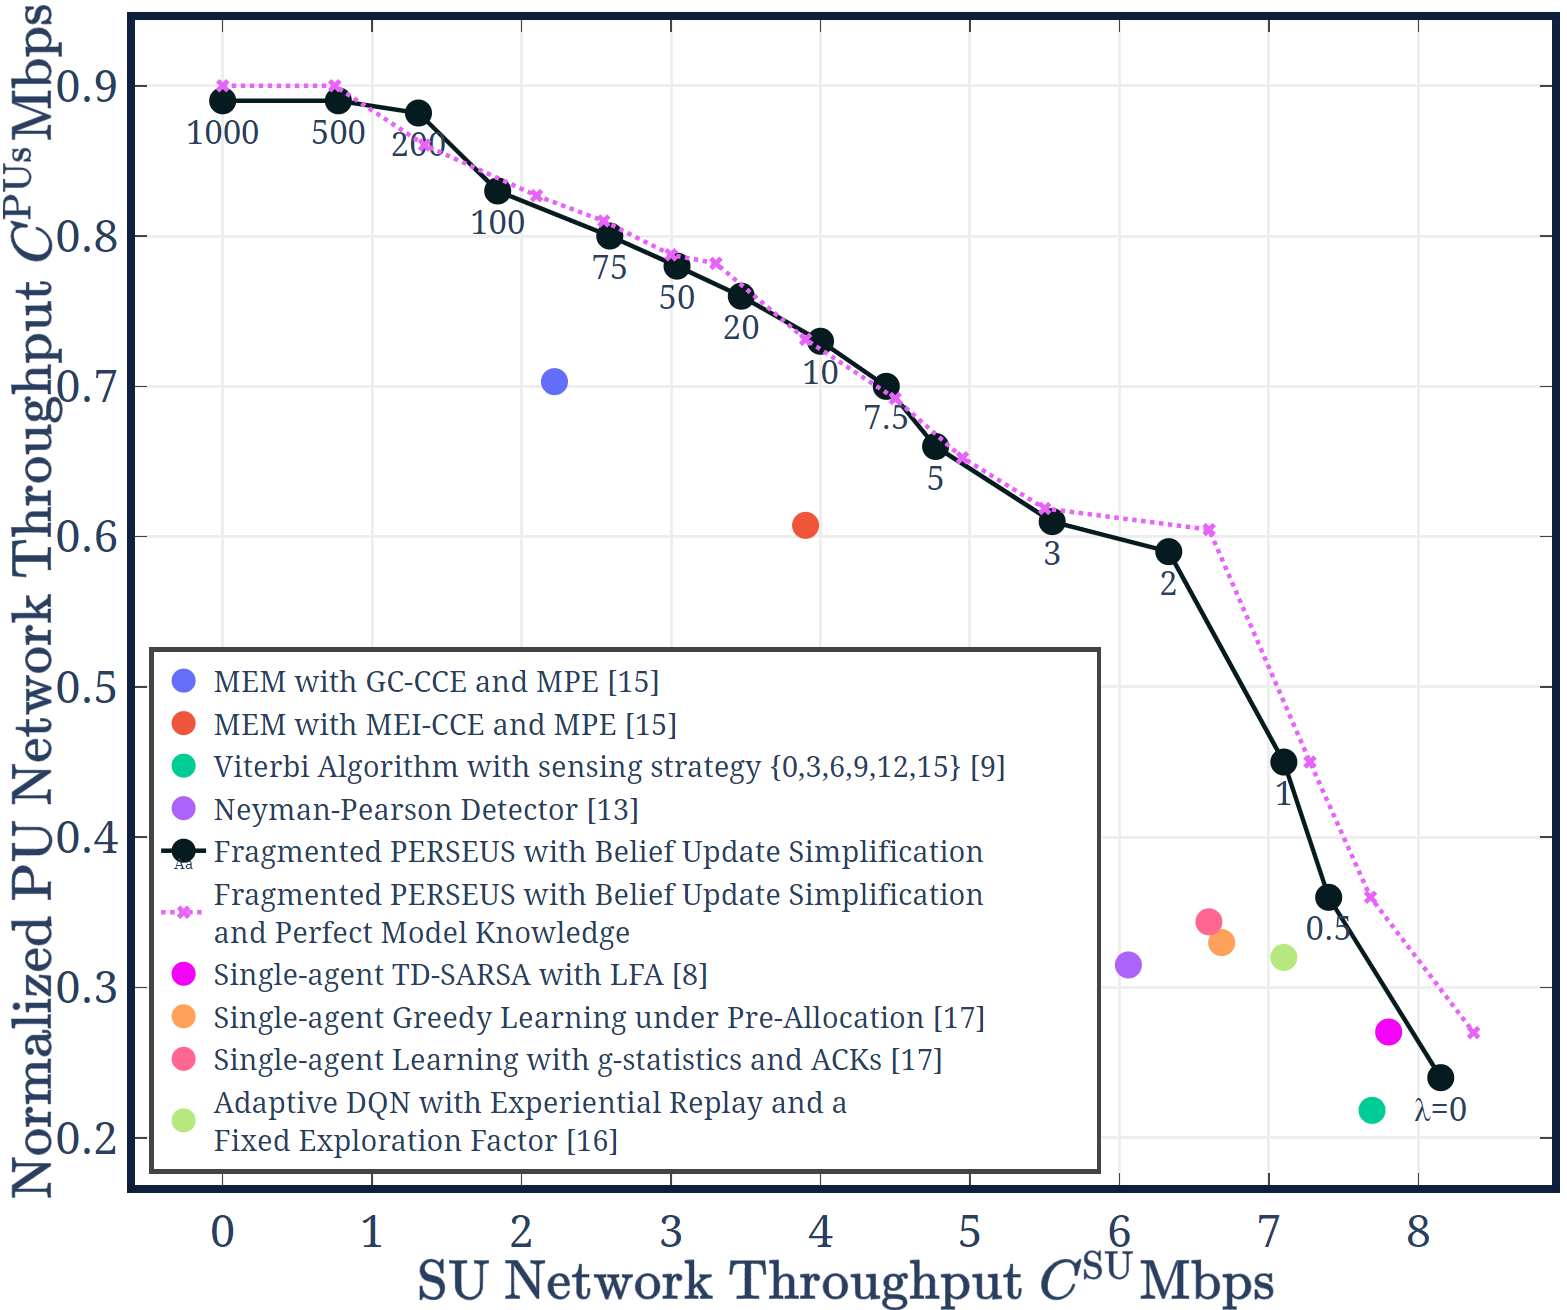
\includegraphics[width = 1.0\linewidth]{figures/Minerva_SoA_Performance_Comparisons_v10.png}}
    \vspace{-6mm}
    \caption{The evaluation of SU and PU network throughputs for different values of $\lambda$, along with comparisons with the state-of-the-art}
    \vspace{-7mm}
    \label{Fig. 4}
\end{figure}

Analyzing the performance of our POMDP solution from a different perspective, we find that, as illustrated in Fig. \ref{Fig. 5}, our framework obtains an average utility, i.e., $R(\vec{\phi}(i),\hat{\beta}_{i})$ described in Sec. \ref{II.0}, of $11.98$ per time-step $i$, $125$\% higher than that achieved by the MEM with GC-CCE and MPE algorithm from \cite{WCL:7}, $96$\% higher than that achieved by the MEM with MEI-CCE and MPE algorithm from \cite{WCL:7}, and $42$\% more than that attained by the Neyman-Pearson Detector detailed above \cite{WCL:11}. Furthermore, in order to understand how our framework performs against a standard HMM state estimation solution like the Viterbi algorithm described earlier \cite{WCL:6}, especially, one with a priori transition model information and one that senses a maximum of $6$ channels per time-slot (channel sensing restriction of $6$), we compare our solution with this Viterbi agent, and find that the average utility per time-slot obtained by the Viterbi agent (${=}11.78$) is $2$\% lower than ours (${=}11.98$).
\begin{figure} [t]
    \centerline{
    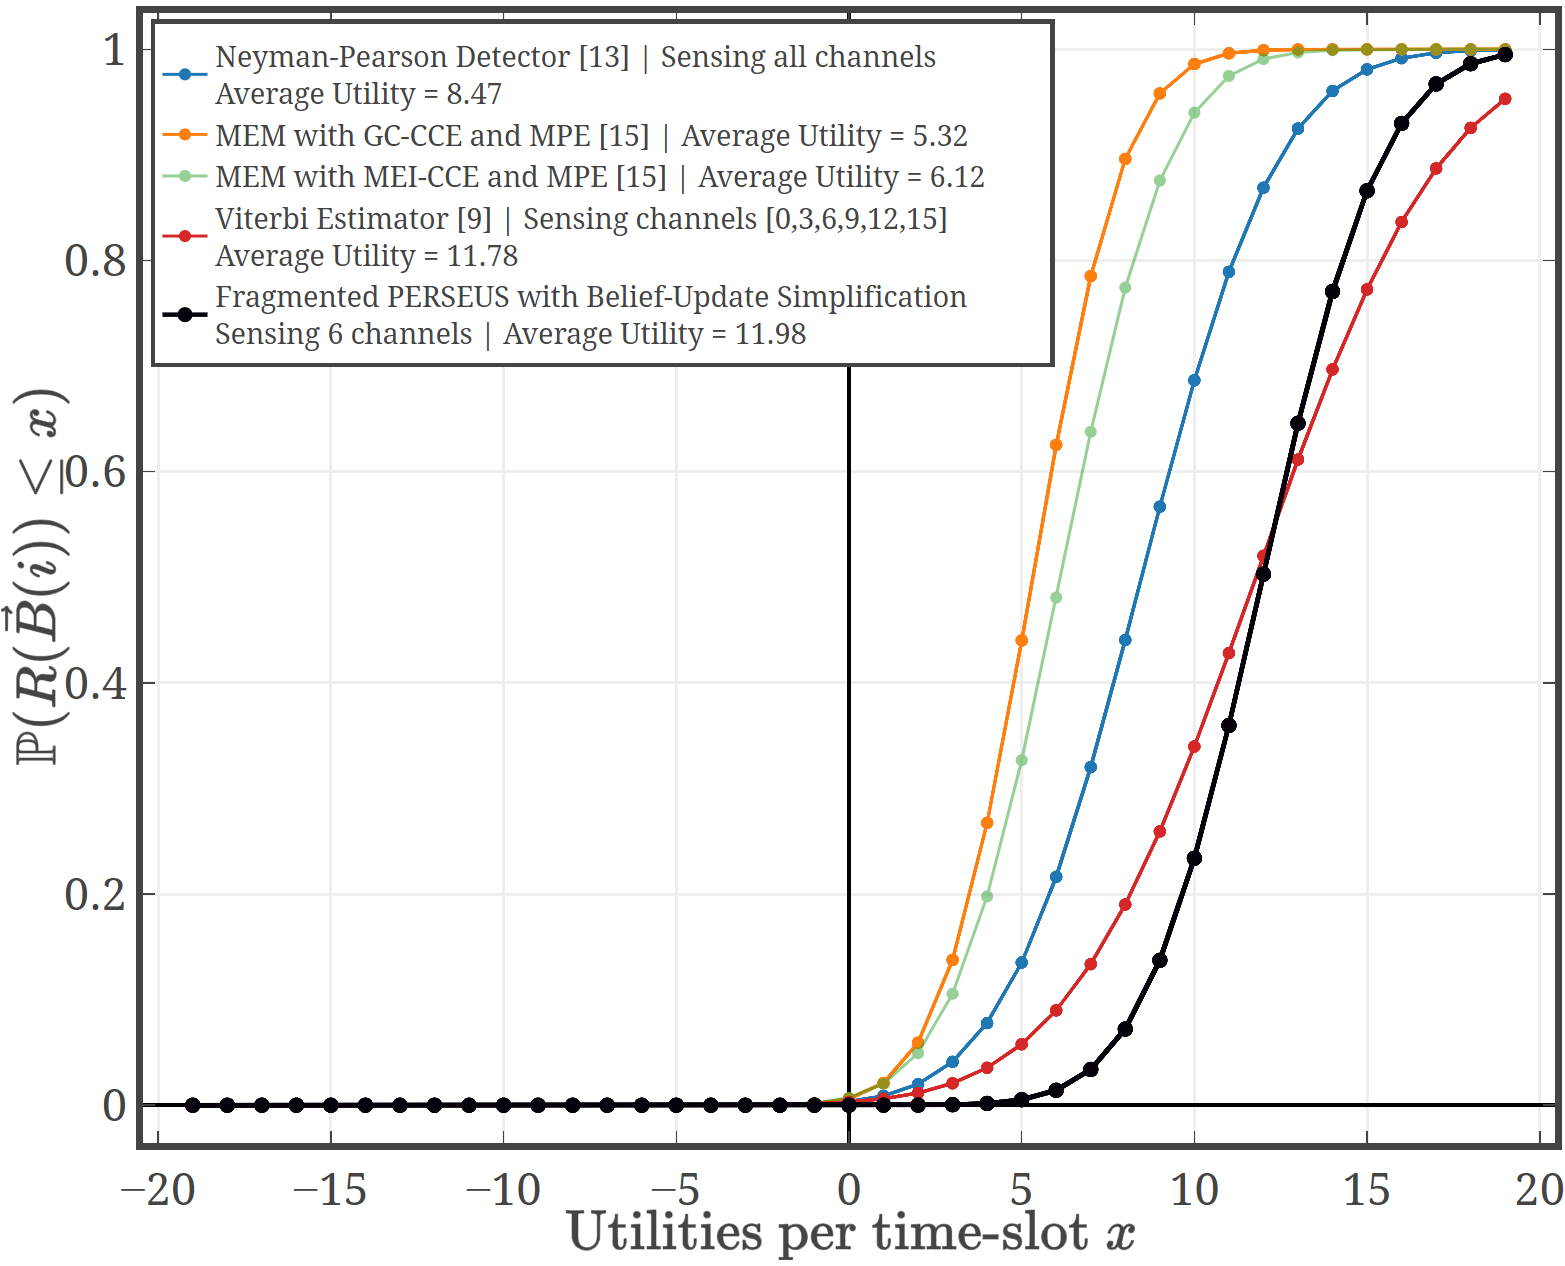
\includegraphics[width = 1.0\linewidth]{figures/Minerva_SoA_Average_Utility_Performance.png}}
    \vspace{-6mm}
    \caption{The evaluation of the proposed solution, from an average utility per time-slot perspective, against a medley of approaches in the state-of-the-art: $\mathbb{P}(R(\vec{B}(i)){\leq}x)$ versus utility per time-slot $x$}
    \vspace{-7mm}
    \label{Fig. 5}
\end{figure}

Specifically discussing the performance of the parameter estimation algorithm, i.e., the HMM EM algorithm (Baum-Welch), we find that, with initial estimates of $0.5$, i.e., $p_{uv}{=}0.5,{\forall}u,v{\in}\{0,1\}$ and $q_{w}{=}0.5,w{\in}\{0,1\}$, the estimator converges to the true parameter vector $\vec{\theta}$ with an error/delta of $\eta{=}10^{-8}$ in $45,000$ iterations: this corresponds to an observation and estimation period of $135$ s, considering a typical time-slot duration of $3$ ms. We illustrate this convergence via the Mean Square Error (MSE) plot depicted in Fig. \ref{Fig. 7}, in which the MSE in iteration $t$ given by,
\begin{equation}\label{32}
    ||\vec{\theta}-\hat{\vec{\theta}}^{(t)}||_{2}^{2}=\sum_{\theta \in \vec{\theta}}\mathbb{E}[(\theta-\hat{\theta}^{(t)})^{2}]
\end{equation}
is decreased iteratively, as the estimation process goes through the E-step and the M-step in each iteration $t$ until $\mathbb{E}[\theta{-}\hat{\theta}^{(t)}]{\leq}10^{-8},{\forall}\theta{\in}\vec{\theta}$.
\begin{figure} [t]
    \centerline{
    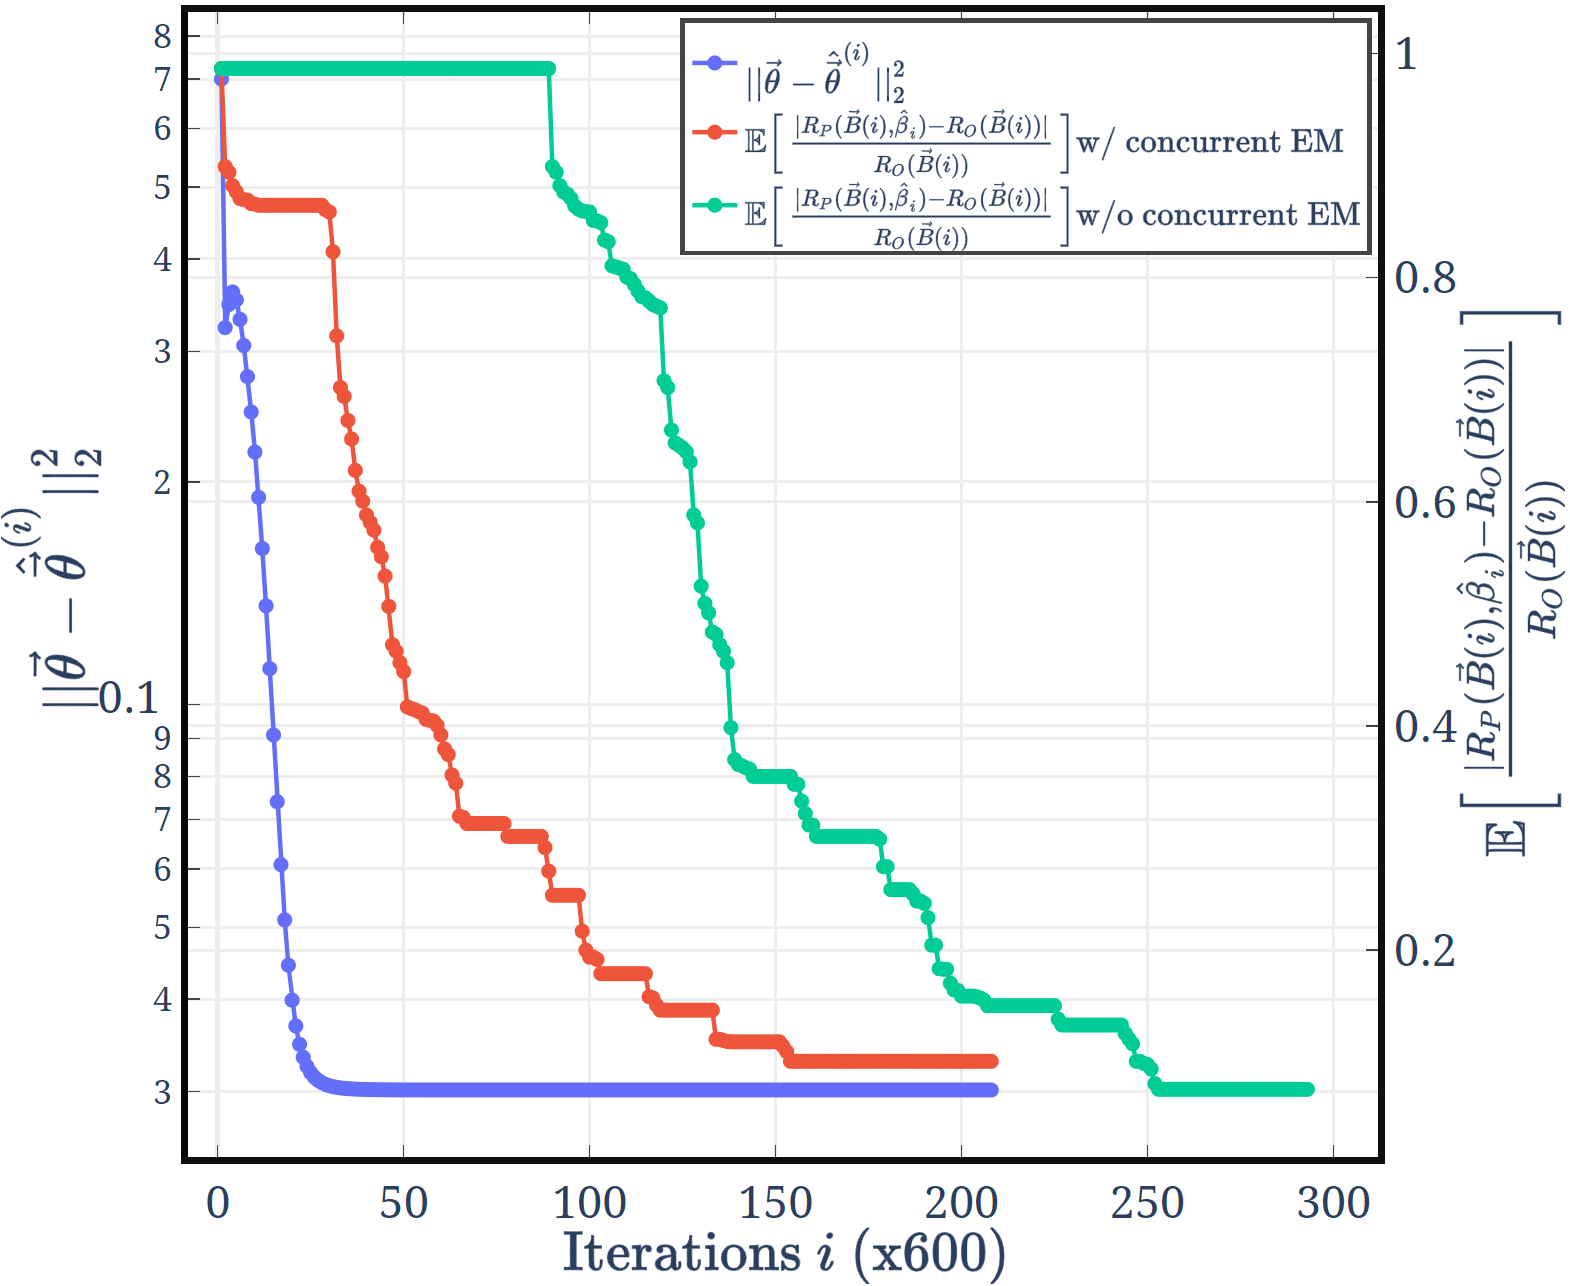
\includegraphics[width = 1.0\linewidth]{figures/Minerva_Computational_Performance.png}}
    \vspace{-6mm}
    \caption{The convergence of the MSE of the HMM EM algorithm to estimate $\vec{\theta}$, and the convergence of the loss of the fragmented PERSEUS algorithm with belief update simplification}
    \vspace{-7mm}
    \label{Fig. 7}
\end{figure}

On the same time-scale as the parameter estimation algorithm, focusing on the loss convergence of the PERSEUS algorithm with a discount factor of $\gamma{=}0.9$ and a termination threshold of $\epsilon{=}10^{-5}$, wherein we define the expected loss as the difference between the utility obtained by the proposed PERSEUS framework, denoted by $R_{P}(\vec{B}(i))$ (discussed in Sec. \ref{II.0}), and that obtained by an Oracle, which knows the exact occupancy behavior of the incumbents in the network, denoted by $R_{O}(\vec{B}(i))$, we find that, as depicted in Fig. \ref{Fig. 7}, the loss convergence of PERSEUS is relatively slower while the parameter estimator is learning the transition model; as opposed to after the convergence of the parameter estimator, when we see a more consistent gradient towards the optimality. Also, note the normalized sub-optimality gap of $0.05$, i.e., the average normalized difference between the utility obtained by our optimal POMDP policy (post-convergence) and the utility obtained by the Oracle (which knows the exact incumbent occupancy behavior) is $0.05$. Moreover, Fig. \ref{Fig. 7} depicts the computational time difference between running the parameter estimator and the PERSEUS algorithm concurrently via the iterative publisher-subscriber architecture, as opposed to initiating the PERSEUS run after the convergence of the parameter estimator: we cut down the time to completion of our HMM-POMDP framework by half by employing the former approach as opposed to the latter, without worsening the sub-optimal gap significantly.

Finally, inspecting Fig. \ref{Fig. 4} in a new light, we see that our POMDP agent limits channel access when the penalty ($\lambda$) is high, leading to lower SU throughput and lower PU interference, and conversely, follows a more lenient channel access strategy when the penalty is low, resulting in higher SU throughput and higher PU interference. Generally speaking, Fig. \ref{Fig. 4} depicts a trend of increasing SU throughput and increasing incumbent interference, as the penalty for missed detections, i.e., $\lambda$ is lowered. Therefore, our framework provides a crucial practical tool in cognitive radio MAC design: the ability to tune the trade-off between the throughput obtained by the cognitive radio and the interference caused by it to incumbent transmissions in the network.

\section{Multi-Agent Deployment Model: An Extension to the single-agent setting}\label{Z}
\subsection{Distributed Multi-Agent Spectrum Sensing and Access}
In this section, we evaluate the performance of the proposed framework: HMM EM + Fragmented PERSEUS with Belief Update Simplification, in distributed multi-agent deployment settings. Operating under the same signal and observation models as in Sec. \ref{I}, consider a network of $3$ PUs operating in an 18-channel radio environment, with their occupancy behaviors in this discretized spectrum of interest governed by Markovian time-frequency correlation structure ($\vec{\theta})$, and $12$ SUs intelligently trying to access white-spaces in the spectrum (cooperatively \cite{WCL:5} or opportunistically \cite{WCL:MIT}), with an added restriction of being able to sense only $1$ channel per SU per time-slot, as illustrated in Fig. \ref{fig: A.0}.

The POMDP model described in Sec. \ref{II.0} has been adapted to this multi-agent deployment setting by incorporating neighbor discovery, channel access rank allocation, and data aggregation algorithms into the original POMDP process flow, as depicted in Fig. \ref{fig: A.add-1}. Designating the band-edges as the control channel, for neighbor discovery, each cognitive radio node broadcasts its control frames (with a frame header and node identifier) over the control channel, and upon receiving control messages from all its surrounding nodes, each cognitive radio node checks if the expected RSSI of the radio signals corresponding to a certain node is above a threshold $\text{RSSI}_\text{th}$: if yes, adds that node’s identifier to its list of neighbors. With a similar control channel strategy for channel access rank allocation, we employ a quorum-based preferential ballot voting scheme to determine the order in which the "estimated-idle" channels are accessed by the SUs in the network. This procedure kicks in only after a quorum has been achieved, i.e., the number of neighbors identified by an SU should be equal to or exceed a node-specific pre-defined number. Over the control channel, each cognitive radio exchanges a ranked list of its neighbors in the decreasing order of their respective  RSSIs, with itself being on the list at position-1 (ties are broken via uniform random choice). Upon receiving an "RSSI-ranked" list from one of its neighbors, each cognitive radio node assigns points to each ranked position, with higher ranks getting larger point values, and re-broadcasts an "aggregated-ranked" list of neighbors (with itself being on the list) with the ranking based on the point-values aggregated across all the ranked lists received from its neighbors (ties are broken via uniform random choice). If the "aggregated-ranked" lists received from its neighbors matches the one at the SU, and this is true for a pre-specified consecutive period of time, a consensus has been reached, the channel access order is determined by this "harmonized-aggregated-ranked" list. If the "aggregated-ranked" lists received from its neighbors differ from the one at the SU, then  the SU repeats the re-ranking of these list members based on their new aggregated point-values and broadcasts the new "aggregated-ranked" list to its neighbors over the control channel. This repetitive process continues until a consensus is reached.

Analyzing the performance of the proposed framework (HMM EM + Fragmented PERSEUS with Belief-Update Simplification) against other distributed multi-agent schemes in the state-of-the-art, as shown in Fig. \ref{fig: Z. 2}, we find that our framework, in terms of the average utility $R(\vec{\phi}(i), \hat{\beta}(i))$ obtained per time-slot, out-performs the distributed, cooperative, $\epsilon$-greedy TD-SARSA with Linear Function Approximation framework from \cite{WCL:5} by $43$\%; out-performs the distributed, cooperative, time-decaying $\epsilon$-greedy algorithm with channel access rank pre-allocations from \cite{WCL:MIT} by $84$\%; and out-performs the distributed, opportunistic, g-statistics algorithm with ACKs (without channel access rank pre-allocations) from \cite{WCL:MIT} by $324$\%.
\begin{figure} [t]
    \centerline{
    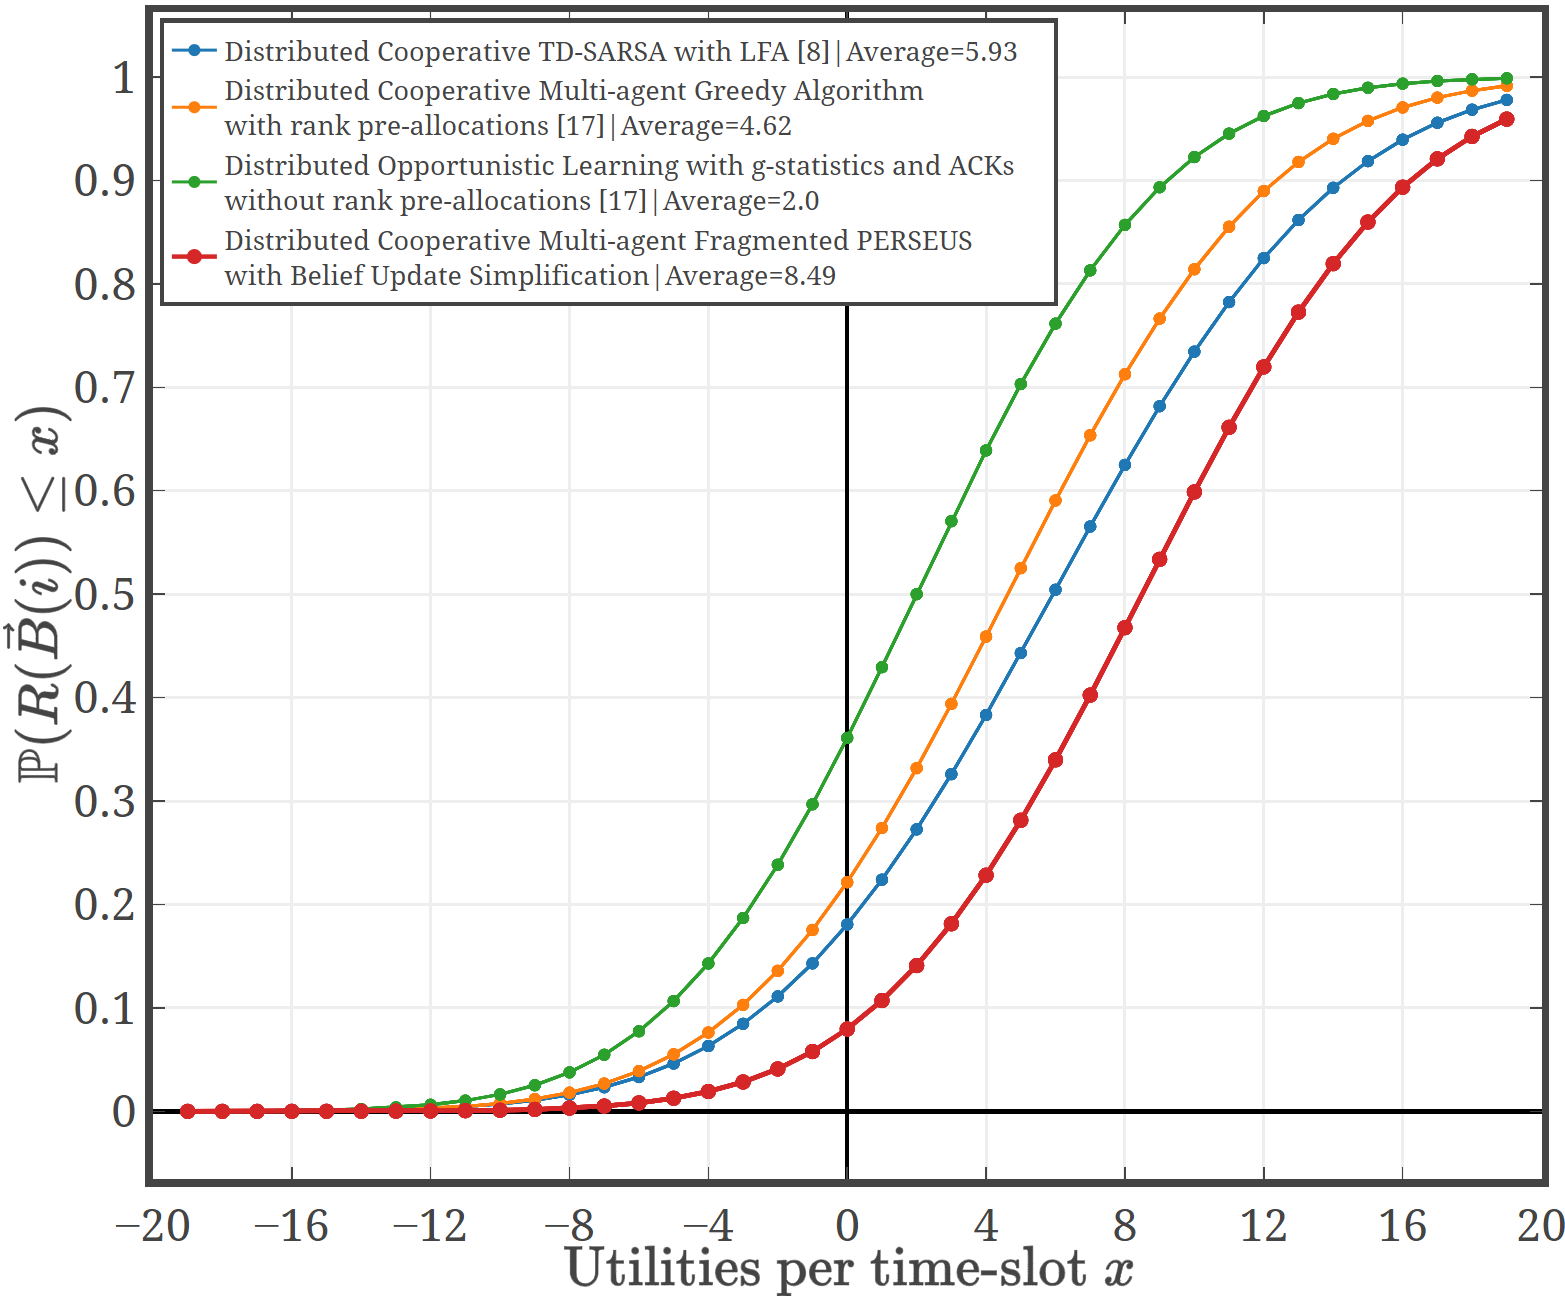
\includegraphics[width = 1.0\linewidth]{figures/Minerva_MultiAgent_SoA_Performance.png}}
    \vspace{-6mm}
    \caption{An evaluation of the performance (average utility per time-slot) of the proposed framework in a distributed multi-agent deployment setting, against other distributed cooperative/opportunistic multi-agent channel sensing \& access frameworks in the state-of-the-art: $\mathbb{P}(R(\vec{B}(i)){\leq}x)$ versus utility per time-slot $x$}
    \vspace{-7mm}
    \label{fig: Z. 2}
\end{figure}

\subsection{Centralized Multi-Agent Spectrum Sensing and Access: SC2 Active Incumbent Emulation}\label{Y}
In order to evaluate the performance of the proposed framework (HMM EM + Fragmented PERSEUS with Belief Update Simplification) in real-world settings, we retrofit it into the MAC layer (channel \& bandwidth allocation) of our BAM! Wireless radio \cite{BAM}, and analyze its operational capabilities in the DARPA SC2 Active Incumbent scenario \cite{DARPA:ActiveIncumbent} emulated on the Colosseum \cite{DARPA:SC2c2api, DARPA:SC2scenarios}. The DARPA SC2 Active Incumbent scenario consists of a Terminal Doppler Weather Radar (TDWR) system functioning as the PU, and $5$ competitor networks (ours included), each constituting $2$ UNII WLANs: $2$ Access Points (APs) and $4$ STAtions (STAs) per AP, serving as the SUs, in a $10$ MHz radio environment ($995$ MHz to $1005$ MHz), for $330$ seconds of emulation on the Colosseum \cite{DARPA:ActiveIncumbent}.

During the Active Incumbent scenario emulation, every competitor network receives network flows from the Colosseum which need to be delivered to the appropriate destination nodes within the network, while satisfying the imposed QoS mandates per flow (for example: max\_latency, min\_throughput, file\_transfer\_deadline, etc.). If the QoS mandates imposed on a particular network flow have been satisfied for a pre-specified period of time (referred to as "Measurement Periods" (MPs)), then the Individual Mandates (IMs) associated with the flow are said to have been met. With this concept of IMs in mind, we can define the points achieved or the "score" of a participant network corresponding to a certain time-slot $i$ as $\sum_{v{\in}\mathcal{V}_{i}} \text{p}_{v}$, where $\mathcal{V}_{i}$ denotes the set of IMs achieved by a participant network in time-slot $i$. The scenario also incorporates ensemble performance thresholds, i.e., all the participant networks should meet the scoring threshold of $8$ \cite{DARPA:ActiveIncumbent}: if a participant network fails to meet this threshold, all the participant networks get the lowest score, i.e., the score corresponding to that achieved by this under-performing network, else, if all the participant networks in the emulation achieve scores that exceed the threshold, their scores are incremented beyond this threshold commensurate with the IMs achieved by them in that time-slot.

After having understood the scoring mechanism involved in the DARPA SC2, we can now evaluate the performance of the proposed framework retrofitted into our standard BAM! Wireless radio \cite{BAM} against other radios designed by our peers who also participated in this competition, in addition to a performance comparison with the weighted PSD + CIL \cite{DARPA:CIL} channel \& bandwidth allocation scheme employed, as a standard out-of-the-box protocol, in our traditional BAM! Wireless network. Leveraging the aggregated PSD measurements obtained at the gateway node of our BAM! Wireless network, as shown in Fig. \ref{fig:A.3} (R), we evaluate the scores of the proposed framework retrofitted into our standard BAM! Wireless radios against our traditional channel \& bandwidth allocation scheme (titled "Standard BAM! Wireless Radio [Purdue]), and against the designs of our peers (identified by their collaboration network registered IP address \cite{DARPA:CIL}, "172.30.210.191 [Peer]" and "172.30.210.181 [Peer]"): in terms of the average score achieved per time-slot, we deduce from Fig. \ref{fig: Y. 4} that the proposed framework ("BAM! Wireless Radio + HMM EM + Fragmented PERSEUS with Belief Update Simplification") out-performs our traditional channel \& bandwidth allocation scheme (a simple weighted PSD + CIL heuristic) by $21$\%; provides a $56$\% better performance than one of our peers, identified by "172.30.210.181"; and attains an $81$\% boost in performance over another one of our peers, identified by "172.30.210.191".
\begin{figure} [t]
    \centerline{
    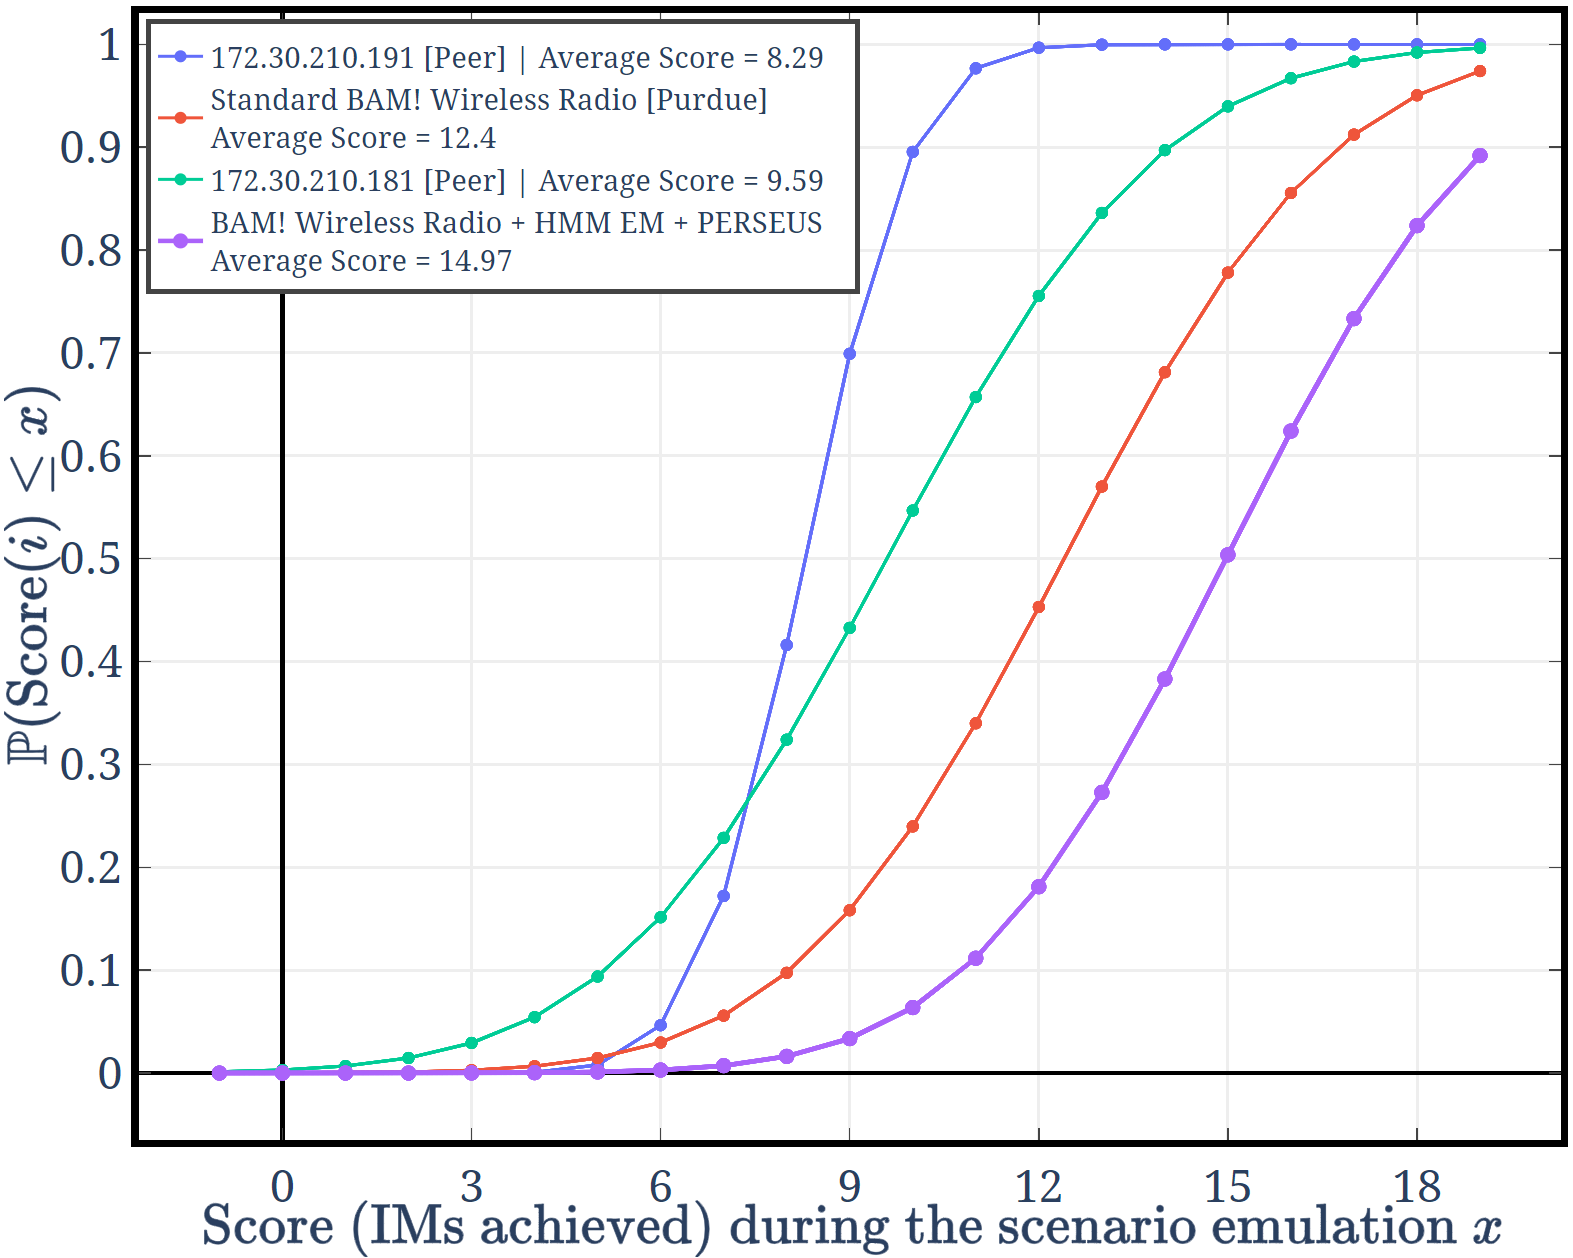
\includegraphics[width = 1.0\linewidth]{figures/Minerva_DARPA_SC2_Performance.png}}
    \vspace{-6mm}
    \caption{An evaluation of the performance (scores/Individual Mandates (IMs) achieved) of our solution by retrofitting the proposed POMDP framework into our BAM! Wireless cognitive radio network design, with respect to an emulation of the DARPA SC2 Active Incumbent scenario, against other competitor network radio designs: $\mathbb{P}(\text{Score}{\leq}x)$ versus the scores achieved during the course of this emulation $x$}
    \vspace{-7mm}
    \label{fig: Y. 4}
\end{figure}

\subsection{Feasibility Analysis of the Distributed Multi-Agent POMDP Optimal Policy on ESP32 Radios}\label{D}
We employ $8$ ESP32 radios \cite{Espressif:ESP32}, with each one embedded in a GCTronic e-puck2 robot \cite{GCTronic:epuck2}, categorized into a network of $3$ PUs (and their $3$ corresponding sinks) occupying $6$ channels in the discretized spectrum of interest according to a Markovian time-frequency correlation structure (described by \eqref{6}), and $2$ independent SUs, with each having the capability of sensing only one channel at a time, intelligently trying to exploit the white-spaces in the spectrum. The detailed methodology of this implementation is provided below:
\begin{itemize}
    \item Considering a network with $J{=}3$ PUs and one SU (work split over $2$ ESP32 radios due to design limitations) with a channel sensing restriction of $\kappa{=}2$ out of $K{=}6$ channels in the discretized spectrum of interest, and assuming a linear AWGN observation model, with a Rayleigh channel fading model (discussed in Sec. \ref{I.I}), we simulate the occupancy behavior of the PUs according to a Markovian time-frequency correlation structure parameterized by $\vec{\theta}{=}[\vec{p},\vec{q}]^{\intercal}$, where $\vec{p}{=}[p_{00}{=}0.1,p_{01}{=}0.3,p_{10}{=}0.3,p_{11}{=}0.7]^{\intercal}$
     and $\vec{q}{=}[q_{0}{=}0.3,q_{1}{=}0.8]^{\intercal}$; and solve for the optimal spectrum sensing and access policy using PERSEUS, embedded with a concurrent parameter estimation algorithm learning the parameter vector $\vec{\theta}$, by mimicking the observational capabilities of the actual ESP32 radios. Note this step is performed on a PC.
    \item The simulated PU occupancy behavior, Markovian correlated according to \eqref{6} and parameterized by $\vec{\theta}$, and the time-slot specific optimal channel access decisions (derived off of the POMDP optimal sensing policy and the simulated PU occupancy behavior), are stored in databases (for export onto the ESP32 network).
    \item Peer-to-Peer communication links are established between a PU ESP32 radio and its sink, using the $3$ ESP32 radios designated as PUs. In other words, $3$ wireless communication links are established: one for each ESP32 PU pair (a source and a sink), over WiFi ($2.4$ GHz) and using a channel according to the occupancy information detailed in the exported PU occupancy database, in time-slot $i$.
    \item Note here that in this ESP32 PU network implementation, in time-slot $i$, while establishing a wireless communication link between a ESP32 PU $j{\in}\{1,2,3\}$ and its respective sink $i{\in}\{1,2,3\}\text{ s.t. }i\text{ is the designated sink for PU }j$, i.e., while forming link $l_{ij}$ over channel $k_{l_{ij}}{=}k{\in}\{1,2,\dots,6\}$ (as determined by the exported PU occupancy database which contains simulated PU occupancy behavior according to the Markovian time-frequency correlation structure described above) such that $k_{l_{ij}}{\neq}k_{l_{i',j'}},{\forall}i,i'{\in}\{1,2,3\},\ j,j'{\in}\{1,2,3\}$, PU $j$ serves as an Access Point (AP) accepting transmission requests from PU $i$, which is designated as a STAtion (STA). In the next synchronized time-slot $i+1$, this link $l_{ij}$ moves to channel $k'{\in}\{1,2,\dots,6\}$, as detailed in the exported PU occupancy database. This same procedure takes place for the other two incumbent communication links in every time-slot until the end of the implementation evaluation period.
    \item Although the PC-based POMDP solver employs an SU which can access $2$ channels at a time in order to deliver its flows (see the access part of the POMDP formulation in Sec. \ref{II.0}), we employ $2$ ESP32 SU radios in the network (serving as one), with the channel access work synchronously and evenly split between the two, due to the actual physical design limitations of the ESP32 radio that it can only access one channel at a time, forcing us to be creative: split the optimal $2$ channel access decision in time-slot $i$, as determined by the time-slot specific optimal POMDP channel access database, into a $1$ channel access action at each ESP32 SU radio. Next, based on whether the channel access at the $2$ ESP32 SU radios was successful, we compute the success rate.
\end{itemize}
The channel access success rate metric defined as
\begin{equation}\label{C.I}
    \text{Channel Access Success Probability}=\frac{\sum_{j=1}^{2}\mathcal{I}\left\{B_{k_{SU_{j}}}(i)=0\right\}}{2},
\end{equation}
where $\mathcal{I}$ corresponding to $\mathcal{I}\left\{B_{k_{SU_{j}}}(i)=0\right\}$ is an indicator variable whose value is $1$ if the channel accessed by the ESP32 SU $j{\in}\{1,2\}$ in time-slot $i$ is not occupied by an incumbent PU ESP32 radio, and $B_{k_{SU_{j}}}{\in}\{0,1\}$ is the occupancy variable of the channel accessed by the ESP32 SU $j$ in time-slot $i$, is evaluated per time-slot $i$, and the resultant channel access success probability is $95.75$\%.

\section{Conclusion}\label{V}
In this paper, we formulate the optimal spectrum sensing and access problem as an approximate POMDP, which leverages learning of the spectrum occupancy correlation model of the incumbents via the Baum-Welch algorithm. Through system simulations, we demonstrate the advantages of exploiting the correlation structure\texttt{-{}-}as opposed to Neyman-Pearson Detector which assumes independence\texttt{-{}-}and of adapting the spectrum sensing decision to optimize the performance\texttt{-{}-}as opposed to Viterbi, which uses a fixed sensing strategy. We also demonstrate the feasibility of a concurrent learning and decision-making framework, as opposed to state-of-the-art correlation-coefficient based clustering algorithms, which rely on pre-loaded datasets for determining the correlation in the incumbent occupancy behavior. Our framework enables a critical feature in practical scenarios: the ability of the SU to regulate the interference caused to PUs, by adjusting a penalty parameter. Also, extending our single-agent model to multi-agent settings, we demonstrate superior performance over the state-of-the-art, in both centralized and distributed deployment settings (collaborative and opportunistic access).
\bibliographystyle{IEEEtran}
\bibliography{ref}
\end{document}